\chapter{\chapivname}
\label{chapter4}
\section*{Overview}
To accomplish pressure mapping with comparable properties to human skin, a novel conductive particle elastomer based sensor device has been created. Using electrical impedance tomography (EIT) to drive a pressure mapping sensor device shows great potential, due to the customisability of the sensing domain and the non-invasive nature of the boundary electrodes required. To translate this research device into a commercial application the performance of such an EIT-based sensor must be quantifiable and repeatable, to be further optimised. In this work a series of experiments on a carbon black silicone rubber sensing domain were repeated for various load locations, strains, and carbon black percentages. Capturing this data gave insight into the how the sensing domain performs over time and captured the transient events limiting the sensor. Metrics were determined to quantify the sensor's spatial resolution. A quasi-static conductance-force model of the material was developed with an accuracy of $\pm$0.78 N. One important metric is temporal resolution, as it is the least quantified performance metric in literature, however can be the most important for some applications. For the sensor domains tested, average settling times of between 19.0 - 44.5 s and 22.5 - 36.0 s were determined for 8 and 9 wt\% CBSR samples. A series of randomised test loads gave similar spatial performance results to the structured experiments. This sensor platform shows promise for future applications, with further materials development and modelling the rise of a biomimetic pressure sensitive skin is imminent.

\footnote{Content from this chapter has been taken from a publication in Sensors and Actuators A: Physical \cite{Ellingham2024}}

\section{Introduction} \label{sec:introduction}
% A poetic start
% Pressure-sensitive biological tissue is critical for humans and animals and has evolved for billions of years to ensure their survival. One of the earliest known animals, the choanoflagellate, required mechanosensation for digestion, locomotion and hence for survival \citep{Maldonado2004}. 

Approximately 1 billion years after the first animals developed mechanosensation \citep{Parfrey2011}, evolution has allowed humans to detect pressure through the use of many mechanoreceptors lying within the skin and other organ tissue. As mentioned in the Literature Review, two mechanoreceptors which are desirable to mimic human touch are Merkel's disks and Meissner's corpuscles \citep{Kamkim2008}. Both of which are ubiquitous in human hands and lips for high spatial resolution, low pressure and low frequency touch/pressure events \citep{Molnar2015}. These mechanoreceptors in a human hand enable object identification and closed loop fine motor control. 

With the creation of pressure mapping technology which has the similar soft mechanical properties and sensing qualities to that of human skin, many applications requiring dexterous human-like touch could be directly fulfilled. This work presents characterisation of a soft mapping pressure sensor which utilises electrical impedance tomography to map resistance changes and subsequently stress changes throughout a soft material surface. 

The number of applications that require 2D pressure sensing using a soft surface is extensive. Such applications include: robotic gripper object detection, medical mattresses and cushions, limb prostheses and wearable robotics, sport equipment, smart furniture, and rehabilitation devices. The following characteristics are desirable for each of these applications: force sensitivity, low toxicity, cost-effectiveness, repeatability, and high elasticity. In this work, a system showcasing each of these desirable characteristics has been developed. 

The sensor platform utilises a piezoresistive nanoparticle elastomer composite (PNEC) in a thin sheet topology to create an artificial sensitive skin. This artificial skin is composed of a highly elastic piezoresistive material, and its deformation can be identified through electrical impedance tomography (EIT) for the reconstruction of the material resistivity image. Using 16 boundary electrodes, EIT facilitates the mapping of applied forces on this monolithic homogeneous material. Subsequently, an inverse model is applied to estimate compressive force loads on the material.

Understanding the electromechanical properties of the PNEC material used in this work is essential for creating an accurate dynamic sensor. When elastomeric composites with conductive particles, such as the PNEC, exhibit viscoelasticity, the degree of hysteresis varies based on the constituents of the composite material \citep{Ellingham2021}. This viscoelasticity is a major limiting factor when using PNECs for EIT-based pressure sensing due to the poor frequency response introduced by the large transient effects seen in the material. In this work these transient phenomena are captured and characterised for 1D and 2D compressive load cases.

% This viscoelastic behavior results in the PNEC material storing elastic energy while also dissipating viscous energy, introducing non-linearity in the stress-strain loading and unloading relationship. Failure to compensate for this resistance-strain non-linearity limits the frequency response of a sensor using PNEC material, constrained by the resistive relaxation time of the material. To address this, the present study focuses on measuring and characterising the transient response of PNEC material in two dimensions, employing EIT reconstruction for two variants of PNEC. To complete such a task in 2 dimensions requires an appropriate sensing technology, and 2D data processing. 

% Leading into the solution + EIT uses and definition
Various methods and topologies of 2D pressure mapping sensors can be employed for a 2D resistivity measurement. However, many of these methods involve intrusive and intricate electrode placement within the material domain \citep{Goncalves2017,Loew2019,Silvera-Tawil2015,Lee2019,Gilanizadehdizaj2022,Zhu2021}. Since the materials utilised in this study are soft, the utilisation of relatively rigid metal electrodes distributed throughout the material would significantly alter the material's electromechanical deformation response. This necessitates use of the non-invasive method imaging method EIT. 

% The selected imaging method for the sensor is Electrical Impedance Tomography (EIT), chosen for its utilisation of boundary electrodes, affordability, simplicity in hardware, and excellent time resolution. EIT has demonstrated superior time resolution compared to other non-invasive medical tomographic imaging techniques \citep{Schullcke2016,Adler2021}. The use of boundary electrodes facilitates pressure mapping of a monolithic material mass while preserving the desirable homogeneous and soft mechanical characteristics of the sensing domain. Although traditionally applied in the biomedical field for non-invasive cross-sectional imaging of physiological tissues and structures within the body \citep{Bayford2018,Hannan2020,Hu2020,Lee2020,Teschner2015}, the EIT method works well with any domain that has an sufficiently low impedance given the limitations of low-cost hardware used in this study.
% TODO?: Mention capacitive sensor equivalents
% cite{Goncalves2017,Loew2019,Silvera-Tawil2015,Lee2019,Gilanizadehdizaj2022,Zhu2021}. 

\subsection{Related Work} \label{sec:Related Work}
Various methods and devices have been designed for localising loads in two-dimensions on a soft domain. A limiting factor found with non-EIT based methods of pressure mapping were the size of discretely sensed regions, also known as sensels. Often these sensels are limited by factors in the fabrication process and the bulk of electrode wires required. This bulk is exemplified high electrode-to-sensel ratio. Example load mapping technology include, optical \citep{Ramuz2012,Shimadera2022,Rossiter2005}, piezoresistive \citep{Gilanizadehdizaj2022,Fu2020,Yang2022}, capacitive \citep{Liang2015}, and magnetic \citep{Yan2021}.


% related works and holes in their research
Other attempts at creating artificial sensitive skins using EIT have been shown in a review by Silvera-Tawil et al. \cite{Silvera-Tawil2015}. This review provides adequate evidence to display a growing interest in the field; however, there is still no commercial EIT-based pressure sensor that is comparable in terms of spatial and temporal resolution, to commercially available non-EIT-based 2D pressure sensors.
One of the earliest applications of EIT to an elastic piezoresistive domain was achieved by Knight and Lipczynski \cite{Knight1990} in 1990. Since this application, several other similar systems have been created using EIT and similar pressure sensitive fabrics or elastomeric materials\cite{Nagakubo2007,Russo2017,Sun2020,Silvera-Tawil2015,Yoon2017,Kato2007,Biasi2022}. A comparison of similar devices is given in Appendix \ref{tab:eit_sensor_compare}. None of these researched devices focus on using a material with similar softness, and quantify the stress data captured in real-time like this work. All of the referenced `EIT' soft sensors employ electrical resistivity tomography (ERT), however, the term ERT is most commonly associated with geological subsurface imaging applications, henceforth, EIT is be used in place of ERT in this work.


\section{Methodology} \label{sec:Methodology}
% high level methodology
To ensure the applicability of Electrical Impedance Tomography (EIT) with a soft PNEC sample, we fabricated the material for testing. The material needed to adhere to specific requirements: highly elastic,  high yield strength, low resistivity, high piezoresistivity, non-toxic, and be a low Shore hardness of 5A - 25A akin to human soft tissue \citep{Silvera-Tawil2015,Chatzistergos2022,McDermott2017,Landry2021}. Additionally, a system of devices was devised to facilitate EIT measurements which concurrently captured force, strain, and timestamps for each measurement. Lastly, to evaluate the sensor's suitability for diverse applications, spatial, temporal, and localised force sensing performance metrics were quantified.


\subsection{Fabrication} \label{sec:Fabrication}
The fabrication of the piezoresistive composite materials, as described and justified in previous chapter and in our previous work \citep{Ellingham2021}, involved dispersing 8 and 9 wt\% of carbon black (CB) nanoparticles in a silicone rubber (SR) matrix. Because of the difference in fabrication processes seen in literature \cite{D'Asaro2017, Shang2016} and degree of dispersion generating variability in the percolation, an iterative trial and error approach using the starting point found in literature was used to get 8 wt \% and 9 wt \% values for CB in SR. Within this range the material was sufficiently conductive while maintaining mechanical strength through sufficient elastomeric cross-linking. Previous research indicates that there is a weight percentage at which the gauge-factor/piezoresistivity is at a maximum within a similar range used in this work \cite{Dong2017, Yang2020}. The composite, designated as the domain under test (DUT), was created using 50 nm average diameter XC 72R CB nanoparticles (Cabot, Alpharetta, USA) in a Dragon Skin 10 NV silicone rubber matrix (SmoothOn, Macungie, USA). Homogeneous dispersion was ensured using an ARV-310 vacuum planetary mixer (Thinky, Tokyo, Japan).
\begin{table}[H]
\caption{DUT mechanical characteristics and electrical characteristics}
\label{tab:DUT_char}
\begin{center}
\begin{tabular}{llll}
\hline
\textbf{Sample}            & \textbf{CB wt} {[}\%{]}    & $\mathbf{R_{int}}$ $[k\Omega]$ & \textbf{E} {[}kPa{]}\\ \hline% & \textbf{Shore Hardness} (ASTM D2240)            \\ \hline
SR        & 0        &         $>1\times10^9$        &       186.16\\
CBSR        & 8        &         $18.1\pm9.8$          &       132.5\\
CBSR        & 9        &         $4.5\pm1.4$           &       98.1\\
\hline
\end{tabular}
\end{center}
\end{table}
The inter-electrode resistance, $R_{int}$, was measured to give an indication of material homogeneity. Elastic modulus, $E$, was calculated from several stress-strain cycles between 0 and 30\%. The $R_{int}$ and $E$ are given in Table \ref{tab:DUT_char}. A CBSR sample developed showing the circular sensitive region with boundary pin electrodes is shown in Figure \ref{fig:CBSR sample and holder}.
\begin{figure}[H]
    \centering
    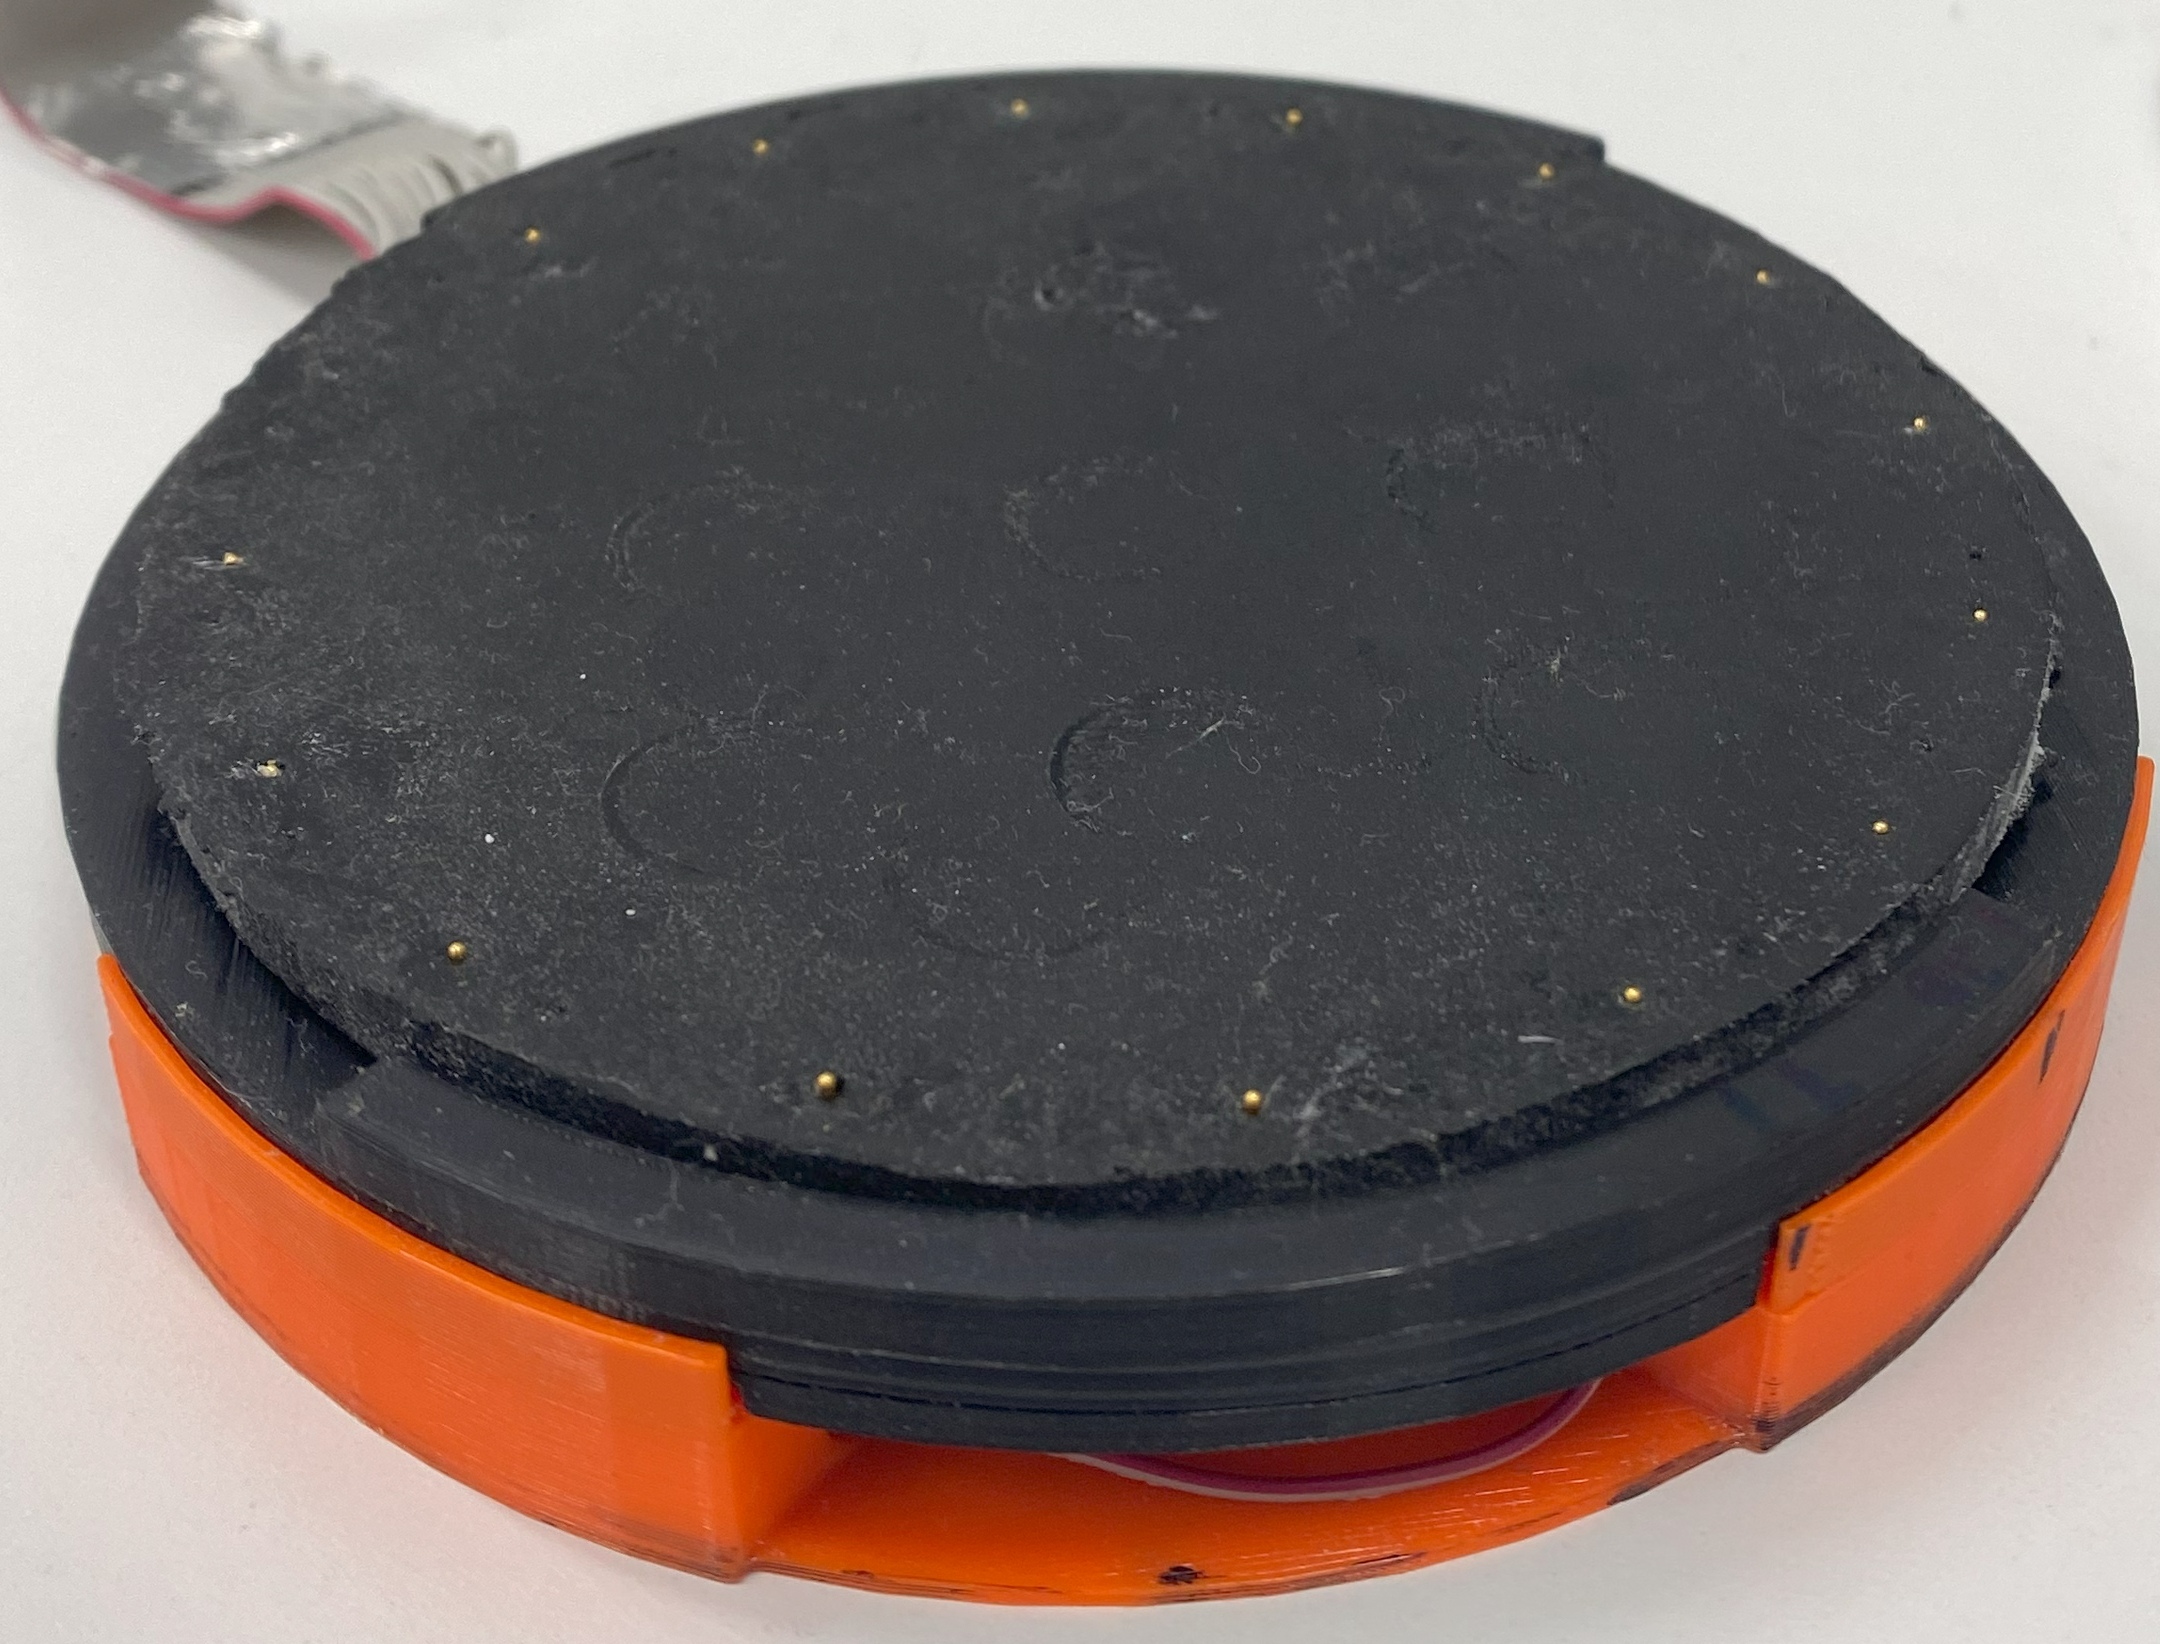
\includegraphics[width=0.3\linewidth]{Figures/CBSR_DUT_w_electrodes_sample.jpg}
    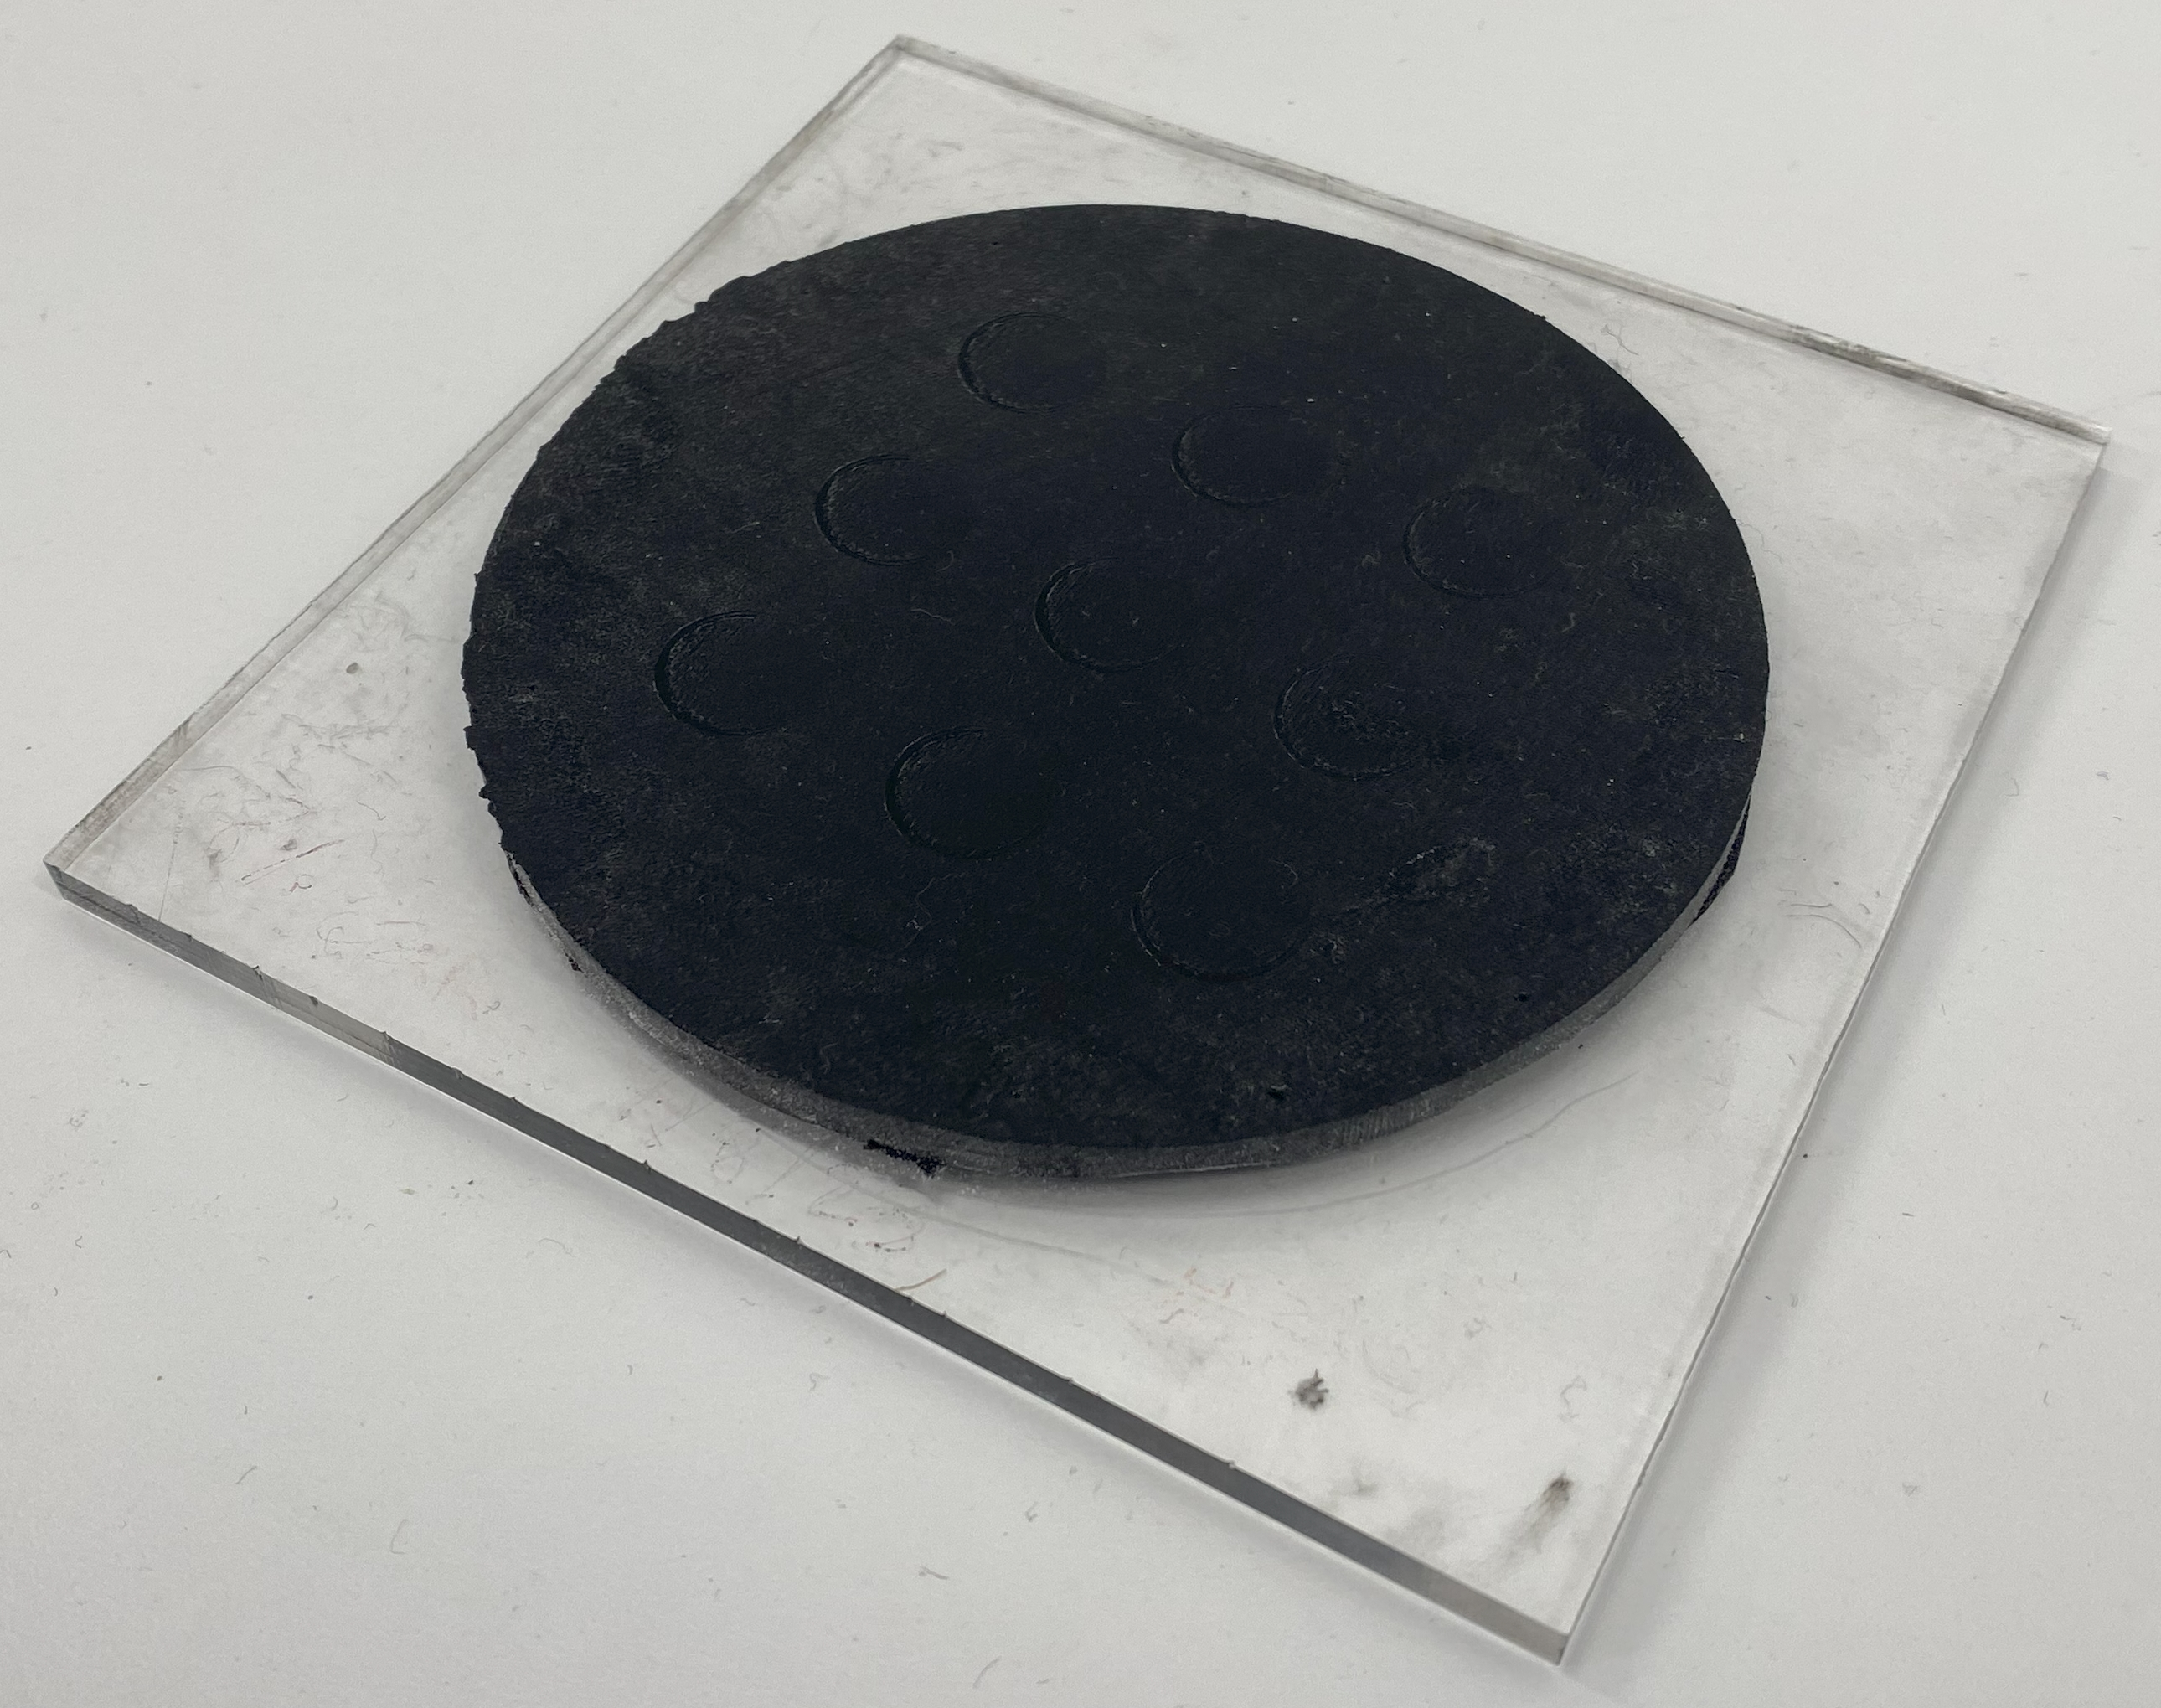
\includegraphics[width=0.3\linewidth]{Figures/CBSR_DUT_sample.jpg}
    \caption{Left: Example of a CBSR sensing domain with gold pin electrodes penetrating material surface around the boundary on top of the rigid sensor holder (orange/black). Right: CBSR sensing domain on an acrylic square.}
    \label{fig:CBSR sample and holder}
\end{figure}

\subsubsection{Localised Stress Testing} \label{sec:Localised Stress Testing}
Quantitative results are required for spatial quantification of the EIT image reconstructions. A cylindrical force applicator head with a diameter of 13 mm and area of 133 mm$^2$ was used to apply the nine compressive loads shown in Figure \ref{fig:force_app_map}.
\begin{figure}[H]
    \centering
    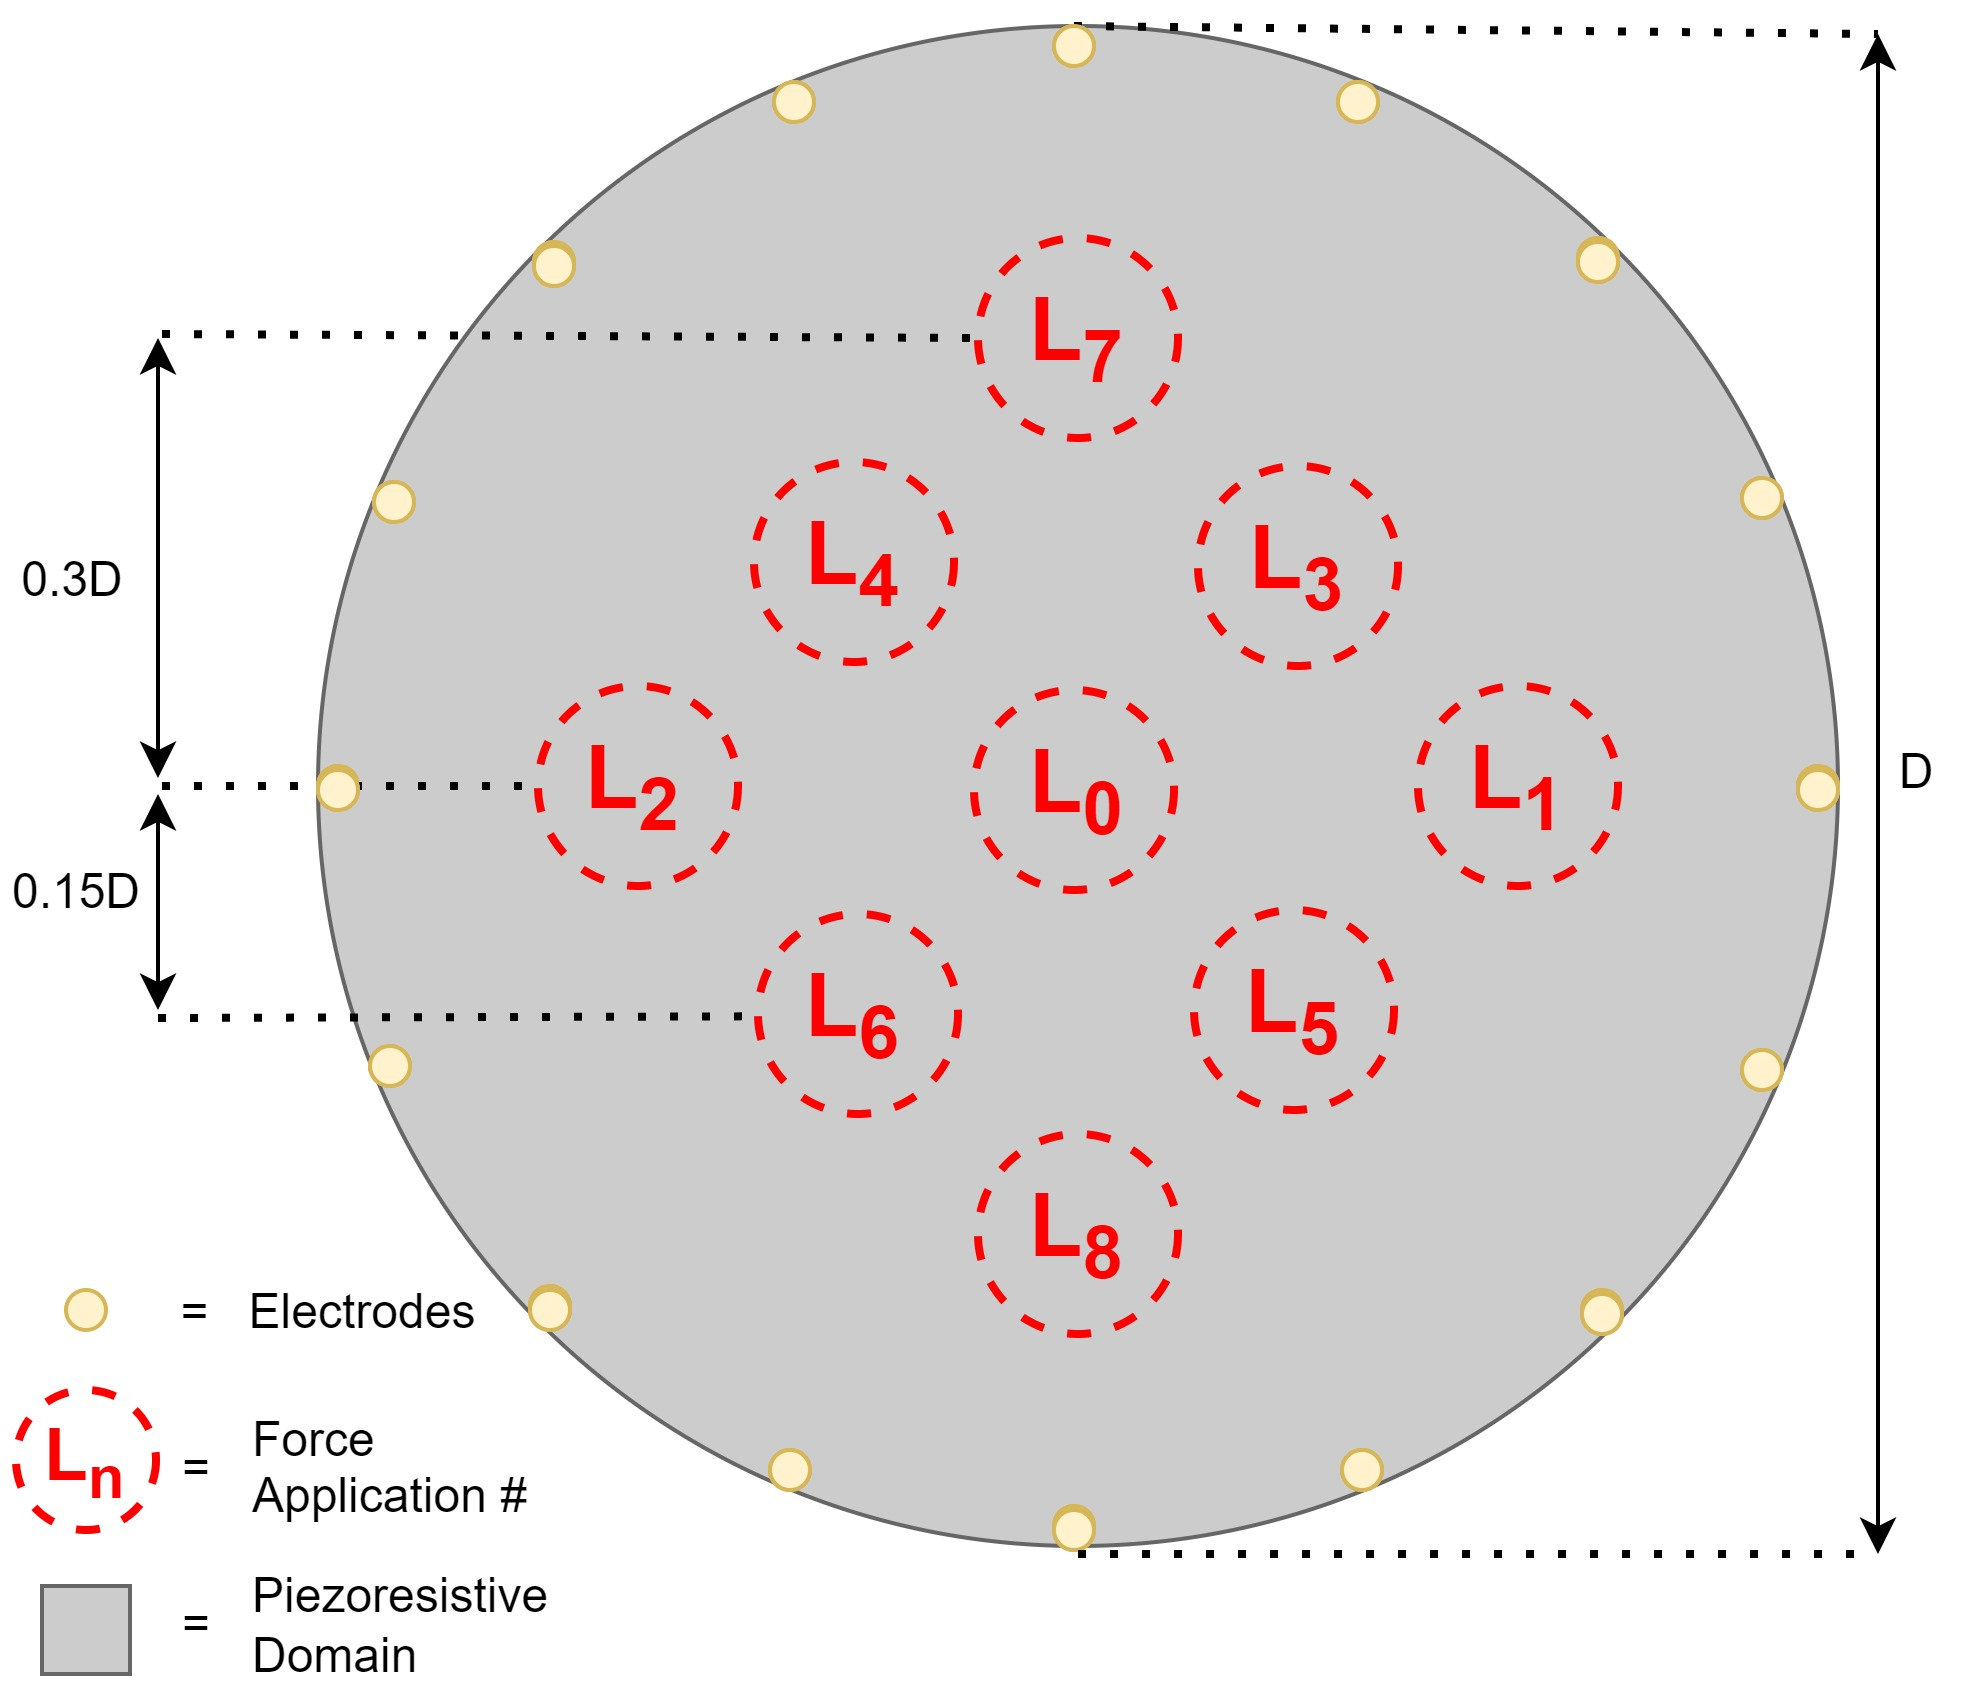
\includegraphics[width=0.6\linewidth]{Figures/EIT_force_app_points_v3.11.jpg}
    \caption{Load application areas used for compressive stress testing shown numerically in order of application.}
    \label{fig:force_app_map}
\end{figure}

\subsubsection{EIT Measurement}\label{sec:EIT Measurement}
EIT data acquisition usually requires a current or voltage source, one or multiple voltmeters, and a switching device. When integrating a mechanical pressure validation system a Cartesian force applicator (CFA) and is also required to capture data simultaneously. The system architecture and DUT electrical connections are shown in Figure \ref{fig:eit_sensor_architecture} and \ref{fig:wiring_ERT_sensor}. This work uses a 2634b source measure unit (SMU) (Keithley, Solon, USA) as a current source and voltage measurement unit for EIT data acquisition. In the following chapter the SMU is miniaturised to a specialised PCB for portable, battery-powered applications.
\begin{figure}[H]
    \centering
    % TODO?: insert a image of the system (tidied up)
    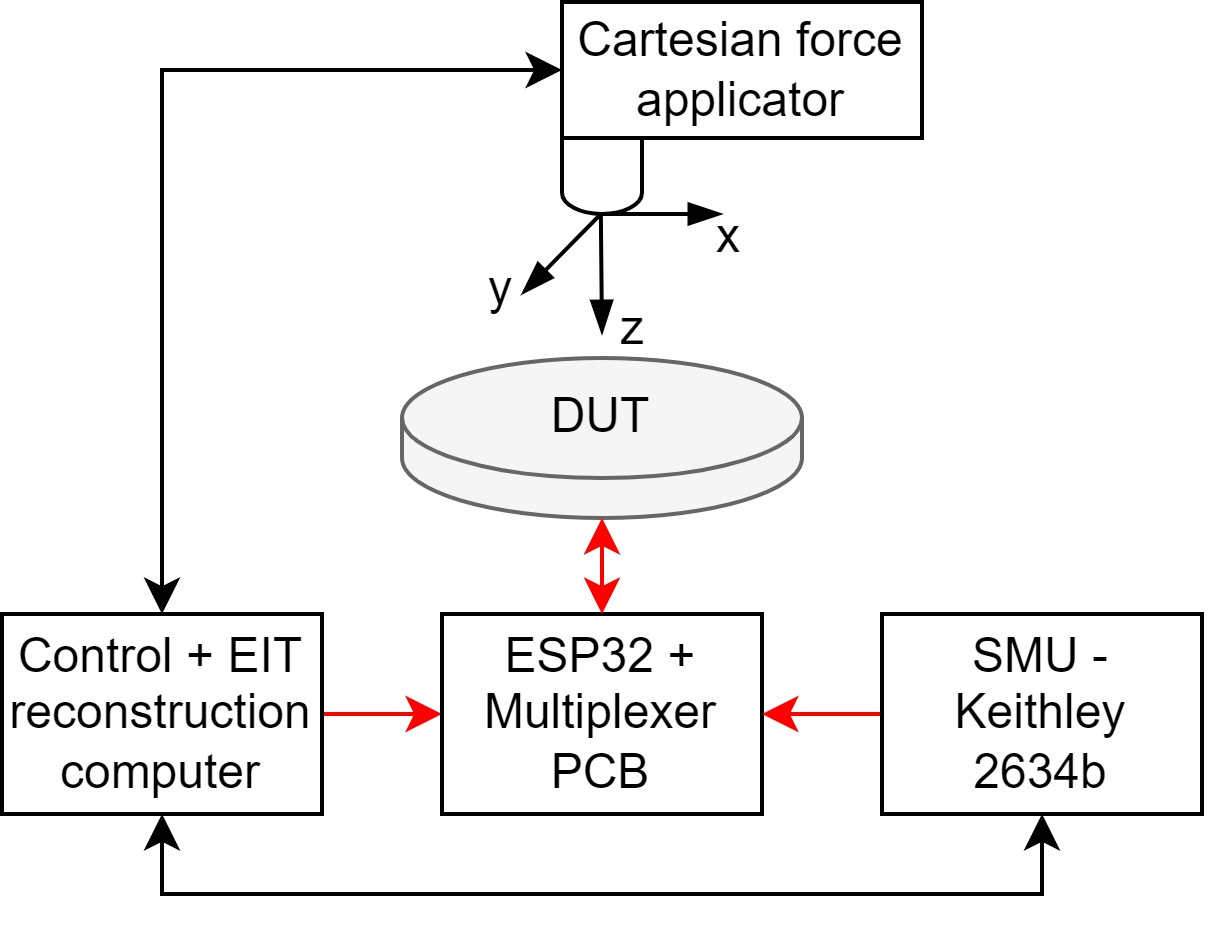
\includegraphics[width=0.6\linewidth]{Figures/ERT_MUX_CFA_architecture.jpg}
    % 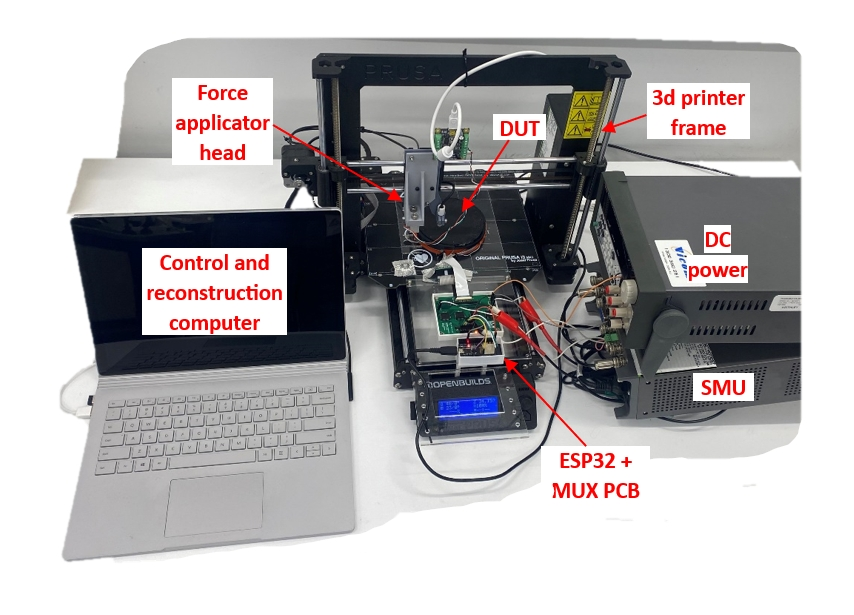
\includegraphics[width=8.5cm]{Figures/cfa_setup_labelled.jpg}
    \caption{Architecture of the Cartesian force applicator setup with red arrows being analogue power lines and black arrows being digital data lines}
    % \caption{Top: Architecture of the Cartesian force applicator setup with red arrows being analogue power lines and black arrows being digital data lines. Bottom: Labelled photo of the EIT sensor and Cartesian force applicator validation system}
    \label{fig:eit_sensor_architecture}
\end{figure}
\begin{figure}[H]
    \centering
    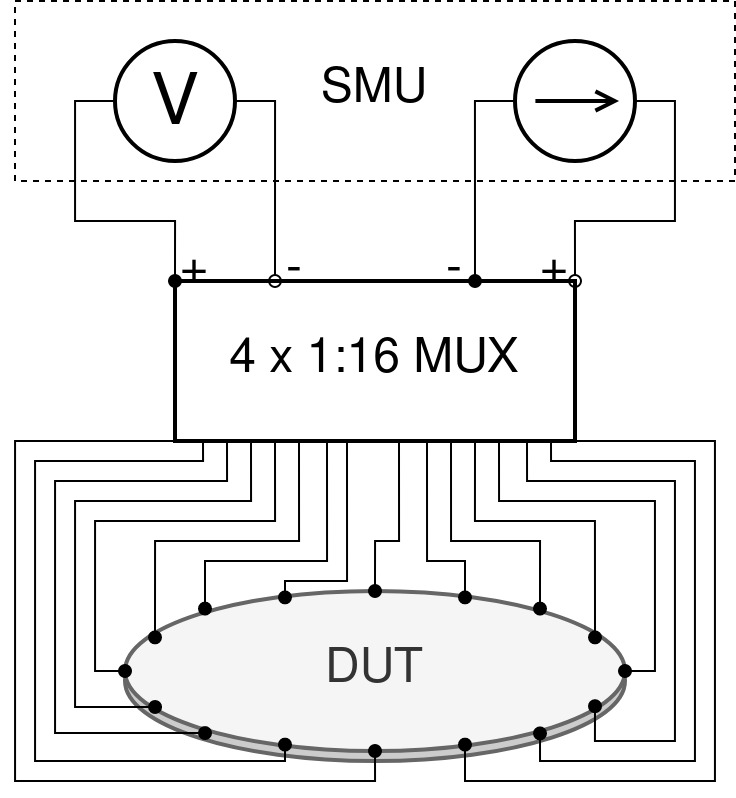
\includegraphics[width=0.35\linewidth]{Figures/wiring_diagram_ERT_sensor.jpg}
    \caption{Wiring diagram for sensor connection to 4:16 multiplexer and SMU}
    \label{fig:wiring_ERT_sensor}
\end{figure} 

% \subsubsection{EIT Solver}\label{sec:EIT Inverse Solver}
% Key parameters for implementing EIT reconstruction included mesh parameters, solver regularisation, and algorithms for reconstructing DUT resistivity. Mesh refinement increased resistivity accuracy near electrode boundaries. The chosen algorithm was the Newton One Step Reconstruction (NOSER) method through EIDORS \citep{Adler1996}, known for speed and accuracy in EIT research. An initial hyper-parameter, $\lambda$, of 0.03 was selected based on positive correlations observed between reconstructions and pressure event contact points.
% TODO?: further reconstruction optimisation can be done for the hyperparameter a set of data. Maybe for each material or each sample?
% TODO?: Insert EIT parameter justification list!


\subsection{1D Material Characterisation} \label{sec:1D Material Characterisation}
Prior to utilising CBSR materials as a 2D pressure sensor, the piezoresistive properties were analysed in one dimension to establish resistance-stress/strain relationships for each CBSR sample. This 1D material testing was conducted using the Cartesian force applicator in conjunction with the SMU. The stress-strain relationship of the material was determined in previous work and shown in Table \ref{tab:DUT_char}. The 1D analysis gave quantitative insight into the material resistivity response to strain in different known areas of the Domain Under Test (DUT) and aligned with the phenomena characterised in the previous chapter, Section \ref{subsec:Quasi-Static Tensile Resistance-Strain}.

\subsubsection{Quasi-static Piezoresistivity}\label{sec:Quasi-static Piezoresistivity}
To determine the piezoresistivity or gauge factor of the material, pin electrodes were pierced through the CBSR samples so that the pin electrodes were parallel and at a distance of 35 mm from each other. The pins were 2.5 mm from each end of the sample. A 2634b SMU was used to apply a constant current of 1 mA between the two pin electrodes while ten compressive loading cycles were applied. The ten loading cycles were applied at strains of 5, 10, 15, 20, 25, and 30\%, with a duty cycle of 50\% and period of 120 s. Loads were applied using the Cartesian force applicator with a 20 mm x 20 mm square flat force applicator head. The strain rate was kept at a constant 16.67$\% \cdot s^{-1}$ to dampen the amplitude of transient effects as proven in previous work \citep{Ellingham2021}.

\begin{figure}[H]
	\centering
	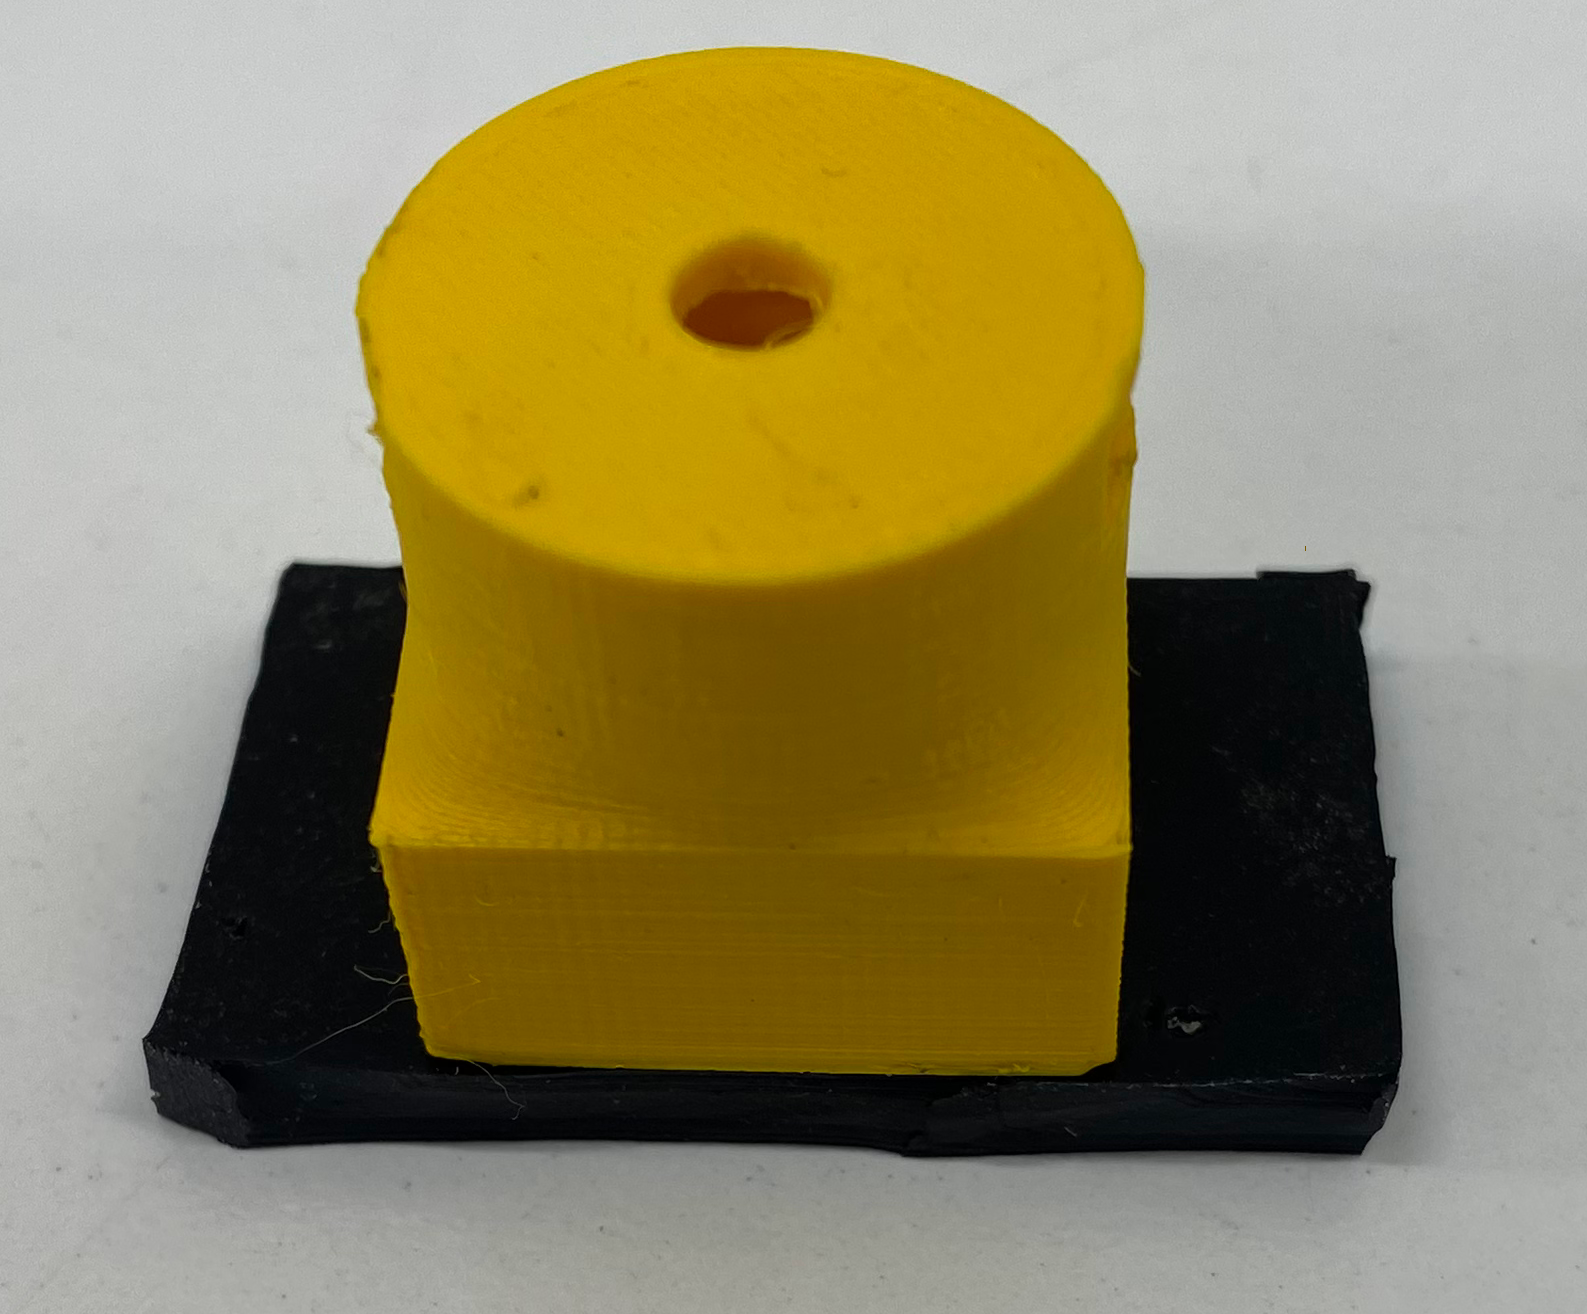
\includegraphics[width=0.25\linewidth]{Figures/QS_load_applicator.png}
	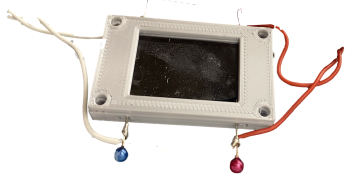
\includegraphics[width=0.4\linewidth]{Figures/QS_load_applicator_w_pins.png}
	\caption{Compressive loading force applicator. Left: Load applicator on sample CBSR material. Right: Pin electrode jig for sample CBSR material compressive loading test.}
	\label{fig:compressive_CBSR_load}
\end{figure}  

When using this material to estimate stress based on resistance, any transient effects that are not correlated between resistance and stress must be accounted for. To obtain a stress reading from this PNEC CBSR material using the quasi-static model given in Equations \ref{eqn:quasi_rstress} and \ref{eqn:quasi_rstrain}, transient events were ignored, so only the steady-state conductance of the material was utilised. 
\begin{equation}
    \frac{\Delta \rho}{\rho_0} = \alpha_\sigma \sigma + \beta_\sigma
    \label{eqn:quasi_rstress}
\end{equation}
\begin{equation}
    \frac{\Delta \rho}{\rho_0} = \alpha_\varepsilon \varepsilon + \beta_\varepsilon
    \label{eqn:quasi_rstrain}
\end{equation}
Where $\alpha$ and $\beta$ are the linear fit parameters, $\sigma$ is the compressive stress, $\varepsilon$ is the strain, $\Delta \rho$ is the change in conductance, and $\rho_0$ is the original material conductance.

\subsubsection{Transient Piezoresistivity}\label{sec:Transient Piezoresistivity}
There are two main piezoresistive events that occur during these compressive stress pulse response experiments. They are the compressive loading and unloading transients. Both of which result in stress relaxation and resistance relaxation behaviour until a steady-state resistance is reached. The stress relaxation can be approximated by a generalised Kelvin linear viscoelastic model \citep{Ju2022} as shown in the previous chapter Section \ref{subsec:resistive relaxation Fitting}. A two component model was found to fit all curves without overfitting, the relaxation model from a step input is given in Equation \ref{eqn:kelvin_general_n2}.
\begin{equation}
    G_2(t) = a_o + a_1 e^{-t/\tau_1} + a_2 e^{-t/\tau_2}
    \label{eqn:kelvin_general_n2}
\end{equation}
Where $G_2(t)$ is the stress relaxation function, $a_0$ is the relaxation offset, $a_1$ \& $a_2$ are the magnitude weightings for each time constant $\tau_1$ \& $\tau_2$. Equation \ref{eqn:kelvin_general_n2} derived from the generalised Kelvin viscoelastic model was used analogously for the resistance relaxation. % TODO?: justify?
To ensure repeatability of the experiment the ten loading and unloading events were fitted using equation \ref{eqn:kelvin_general_n2} to the each relaxation, then the $R^2$ goodness of fit was compared for all of the relaxations.
% TODO?: explain why there are outliers. Due to noise error and the nature of the fitting algorithn LM-LS??

An important temporal characteristic of this system is the settling time, $t_s$, given a strain step input. In this system the resistance step response settling time was the time taken to reach and stay within a specified tolerance about final steady-state resistance, given a strain step input. The tolerance chosen is about the steady state was $\pm$ 15\%. % When using this settling time to gather sensor data, if the tolerance is increased the response time decreases and the sensor force accuracy decreases, vice versa for a decreased tolerance. 
% Below is not valid for our system >>
% For a first order system after 3 time constants a tolerance of $\pm$15\% about the steady-state will always be achieved. Using dominant pole approximation the settling time was calculated. The requirement for the dominant pole approximation were: $\tau_2 / \tau_1 \geq 5$, given $\tau_1 < \tau_2$. This was compared to actual settling time, $\tau_{act}$ for the fitting solutions to reach $\pm 5\%$ of steady-state.
% https://courses.engr.illinois.edu/ece486/fa2021/documentation/lectures/slides/Lecture10A_DominantPoleApproximation.pdf

\subsection{Sensor Performance Metrics}\label{sec:Sensor Performance Metrics}
To ensure that the resistance/conductance image reconstructions which will form stress maps are valid solutions, the quality of the reconstructions needs to be quantified computationally. The purpose of this section is to describe various metrics used for sensor validation. These metrics measure the spatial performance, temporal performance, and localised force sensing performance. Many of the spatial and temporal performance metrics have been taken and adapted from Adler et al. \citep{Adler2009} and their GREIT (Graz consensus Reconstruction algorithm for EIT) performance metrics.

\subsubsection{Pre-processing}\label{Pre-processing}
To ascertain the occurrence of a piezoresistive event in the material, it is necessary to identify a change in resistivity that surpasses the noise floor level. This precaution is taken to differentiate between a stress compression event and potential noise artefacts. A threshold was established to eliminate the noise floor, thereby isolating the loading signal and any noise or artefacts generated by the loading signal(s).

A second threshold filter was implemented to compensate for the regularisation of the reconstruction using a percentage of the largest peak observed in the sensor image domain. The percentage threshold value used in previous work has been 25, 50, 60, 70, 75\% of the maximum domain amplitude \citep{Adler2009,Visentin2016,Silvera-Tawil2015}. In this work percentage threshold masking have been applied for comparison. To validate the best percentage threshold, these thresholds were completed for a CBSR 8 and 9 wt\% PNEC under nine successive loading events comparing the mean of the three main performance metrics given in Section \ref{sec:Spatial Performance}. After these threshold masks have been applied to the 2D EIT images, blob(s) are observed as the sensed regions-of-interest. In this work the term `blob' refers to an amorphous 2D shape made of several aggregated finite mesh elements. These blobs are usually observed after percentage threshold masking of an EIT image reconstruction. 

\subsubsection{Spatial Performance}\label{sec:Spatial Performance}
The three main metrics of spatial performance are the centroid or centre of `mass' error, $E_{CoM}$, the detected area overlap $A_{OL}$ value, and the fit of the detected blob relative to the force input, the shape distortion, $S\!D$.

The $E_{CoM}$ was found using:
\begin{equation}
    E_{CoM} = \sum_i^{N_{b}} e_{{CoM}_i} \times \frac{e_i}{e_{total}}
    \label{eqn:err_CoM}
\end{equation}
Where $N_{b}$ is the number of elements in the threshold masked blob, $e_{{CoM}_i}$ is each individual element centroid, $e_i$ is the $i^{th}$ blob element resistance value and $e_{total}$ is the sum of all of the blob element resistance values. This equation can be easily be inverted for images containing conductance elements in place of resistance elements. The nearer the $E_{CoM}$ value is to zero, the better the reconstruction in regards to localising the sensed region.

The $A_{OL}$ was found using:
\begin{equation}
    A_{OL} = 100\times\left[\frac{\left(\sum_i^{N_{b}} A_{e_i}\right)}{A_{FA}} + \frac{\left(\sum_i^{N_{b}} A_{e_i}\right)}{A_{b}}\right]\bigg/2 : e_{{CoM}_i} \in \Omega_{FA}
    \label{eqn:area_overlap}
\end{equation}
Where $A_{e_i}$ is the area of an element and $\Omega_{FA}$ is the domain of the force applicator area. $A_{FA}$ and $A_{b}$ are the areas of the force applicator and sensed region respectively. The closer the $A_{OL}$ is to 100\%, the more overlap there is between the estimated and actual load application.

The $S\!D$ was found using:
\begin{equation}
    S\!D = \left[\sum_j^{N_p} \left(\|F_{CoM} - P_j\|_2 - r_{FA}\right)^2\right] \bigg/ N_p : P_j \in L_{b}
    \label{eqn:shape_deform}
\end{equation}
Where $N_p$ is the number of mesh nodes on the perimeter of the blob, $F_{CoM}$ is the force applicator centre of mass (CoM) coordinates, $P_j$ is a node in the set of blob perimetral nodes, $L_{b}$, and $r_{FA}$ is the radius of the force applicator head. The $S\!D$ is essentially the mean square error of the force applicator perimeter and sensed region perimeter taken radially from the force applicator centroid.


\subsubsection{Temporal Performance}\label{sec:Temporal Performance}
A core problem with using soft PNECs is the temporal resolution they can provide can be limited by the viscoelasticity in the material and how it interacts with the conductive network in the material. This section provides insight into how to determine the frequency response of the material, by observing the relaxation settling time of the material. The maximum time taken to reach a steady-state resistance after a stress event dictates the frequency at which the material can sense stress events. To determine the time taken to reach a steady-state, a variety of compressive stresses and strains at the loading locations, $L_0$-$L_8$, of each DUT are observed. 


To determine whether the resistance relaxation observed in the 1D case matches the relaxation of the reconstruction in 2D, the 1D and 2D relaxation settling times were compared to validate whether similar frequency responses were being observed. The EIT measurement equipment was designed such that the reconstruction frequency of 0.4 Hz can capture these transient events observed triggered in the CBSR samples, which are typically in the order of tens of seconds. 


From the blob localisation described in section \ref{sec:Spatial Performance} the resistance relaxation data was extracted by plotting the sum of the blob resistance. Similar to the 1D case, the relaxations for stress loading, resistance loading, and resistance unloading scenarios are captured and compared for each CBSR with CB weight percentages of 8 and 9 wt\%. The blob resistance relaxation was compared to relaxation deduced from the total image domain resistance to ensure that the only the transient event from the area being loaded was being observed.

\subsubsection{Localised Force Sensing Performance}\label{sec:Localised Force Sensing Performance}
As discussed in Section \ref{sec:Quasi-static Piezoresistivity}, a quasi-static function, Equation \ref{eqn:quasi_rstress}, has been generated that gives a stress based on 1D steady-state conductance measurements. This quasi-static function was applied to the DUT 2D reconstruction to obtain a stress map of the material. To determine the minimum detectable stress of the sensor the conductance noise floor values were input into the linear quasi-static Equation \ref{eqn:quasi_rstress}.

To obtain the stress estimate, $\hat\sigma_j$ and hence force estimate given a known input stress and force, the following steps were completed for each CBSR sample:
\begin{enumerate}
    \item Determine the most likely sensed region:
    \begin{enumerate}
        \item An EIT reconstruction image of a loaded DUT of a particular strain, $\varepsilon_j$, at a steady-state conductance was found. Each element having a change in conductance value, $\Delta\rho$, in units $mS$.
        \item Complete threshold percentage mask on image to localise the sensed region blob(s).
        \item The centre of mass error, $E_{CoM}$, between each blob and the actual force application CoM was calculated. The blob domain with the smallest $E_{CoM}$, $\Omega_s$, is chosen for the following steps.
    \end{enumerate}
    % \item A new mask the shape, size and location of the force applicator + 30\% to compensate for the EIT regularisation is applied to the reconconstruction in step 1 to get a new sensed region, $\Omega_f$. % TODO: Justify this + 30% mathematically.
    \item Equation \ref{eqn:quasi_rstress} was rearranged to get an original conductance estimate for each element:
    \begin{equation}
        \rho_0 = \frac{\Delta \rho}{\alpha \sigma+\beta}
        \label{eqn:C0_est_stress}
    \end{equation}
    \item The mean $\rho_0$ and standard deviation of all of the elements in $\Omega_s$ were found.
    \item Steps 1 to 3 were repeated for each strain, $\varepsilon_j$, applied and the mean, $\rho_0(\varepsilon_j)$ and standard deviation  were calculated.
    \item The mean of all $\rho_0(\varepsilon_j)$ across all strain values (i.e. $\varepsilon_j = 5, 10, 15, 20, 35, 30\%)$ was calculated as $\bar\rho_0$.
    \item $\bar\rho_0$ was then substituted into Equation \ref{eqn:quasi_rstress} as $\rho_0$, which was rearranged for stress to obtain the stress estimate as a function of mean change in conductance, $\hat\sigma_j(\Delta \bar\rho_j)$, of the sensed blob domain, $\Omega_s$.
\end{enumerate}
% TODO: Determine a mathematical justification of the fudge factor which rho_0 is multiplied by.
% TODO: describe how stress limits were found (e.g. noise figure, ringing, more?)


\section{Results}\label{sec: Results}
In the following sections the EIT image pre-processing, spatial, temporal, and localised force sensing performance metrics are displayed and quantified. First the steady state electrical noise, $\sigma_n$, and noise figure, NF, were determined, as given in Table \ref{tab:DUT_noise}. The NF value is a common metric showing noise amplification as a consequence of the EIT algorithm as used by Adler et al \citep{Adler2009}.
\begin{table}[H]
\caption{DUT noise figure, NF, and noise, $\sigma_n$, at steady-state}
\label{tab:DUT_noise}
\begin{center}
\begin{tabular}{p{2cm}p{2cm}p{2cm}}
\hline
\textbf{CB wt\%} & \textbf{NF} & $\sigma_n$ [mS]\\ \hline
8           & 1.20 $\pm$ 0.17 & 0.69         \\
9           & 1.15 $\pm$ 0.11 & 0.48            \\ 
\hline
\end{tabular}
\end{center}
\end{table}


\subsection{1D Material Characterisation} \label{sec:1D Material Characterisation2}
To generate a 2D pressure map from the EIT reconstructions a 1D material electromechanical characterisation was required. The 1D electromechanical relationship can then be extended to form an electromechanical relationship in 2D.

% \subsubsection{Stress-strain}\label{sec:Stress-strain2}
% Given known strain inputs and measured stress output data the elastic modulus of the CBSR 8 wt\% and 9 wt\% data was calculated as 132.5 kPa and 98.1 kPa respectively.
% \begin{figure}[H]
%     \centering
%     \includegraphics[width=8cm]{Figures/CBSR 8wt 9wt stress-strain.jpg}
%     \caption{Stress strain data and fitted curves for 8 wt\% and 9 wt\% CBSR composites.}
%     \label{fig:stress-strain}
% \end{figure}
% TODO?: Append plot and put both plots into paper

\subsubsection{Quasi-static Piezoresistivity}\label{sec:Quasi-static Piezoresistivity2}
Given known strain input data, and measured stress and conductance change output data, a fit is shown in Figure \ref{fig:quasi_r_8p}. The gradient of the linear fit, i.e. the gauge factor, for the CBSR 8 wt\% and 9 wt\% was calculated as 0.6 and 0.2 respectively. Note that in the 9 wt\% relative conductance data the standard deviation of the 5\% strain data was similar to that of the mean, hence the linear range of 10 - 30\% strain was considered when fitting the curve.
\begin{figure}[H]
    \centering
    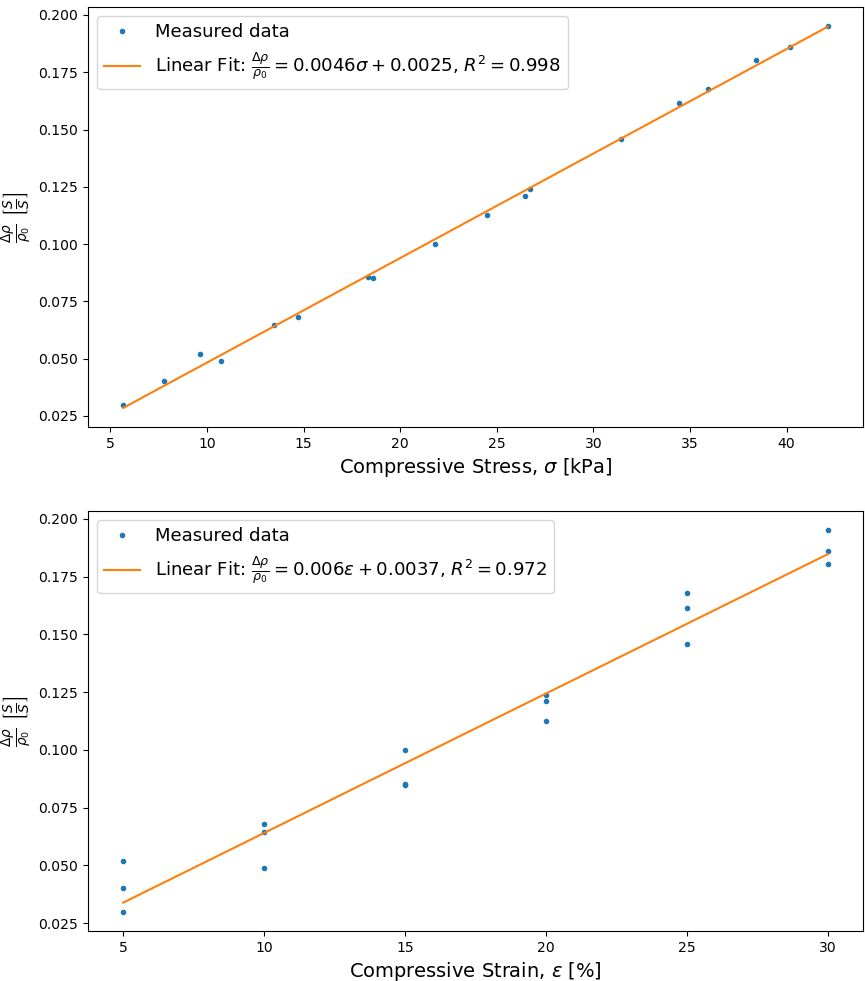
\includegraphics[width=0.8\linewidth]{Figures/CBSR_8p_cond_stress_strain_sin_titulo.jpg}
    \caption{Conductance change vs. stress (top) and strain (bottom) data and fitted curves for 8 wt\% CBSR.}
    % TODO?: Change Linear fit to 10^{-1} from 10^{-3}
    \label{fig:quasi_r_8p}
\end{figure}
% \begin{figure}[H]
%     \centering
%     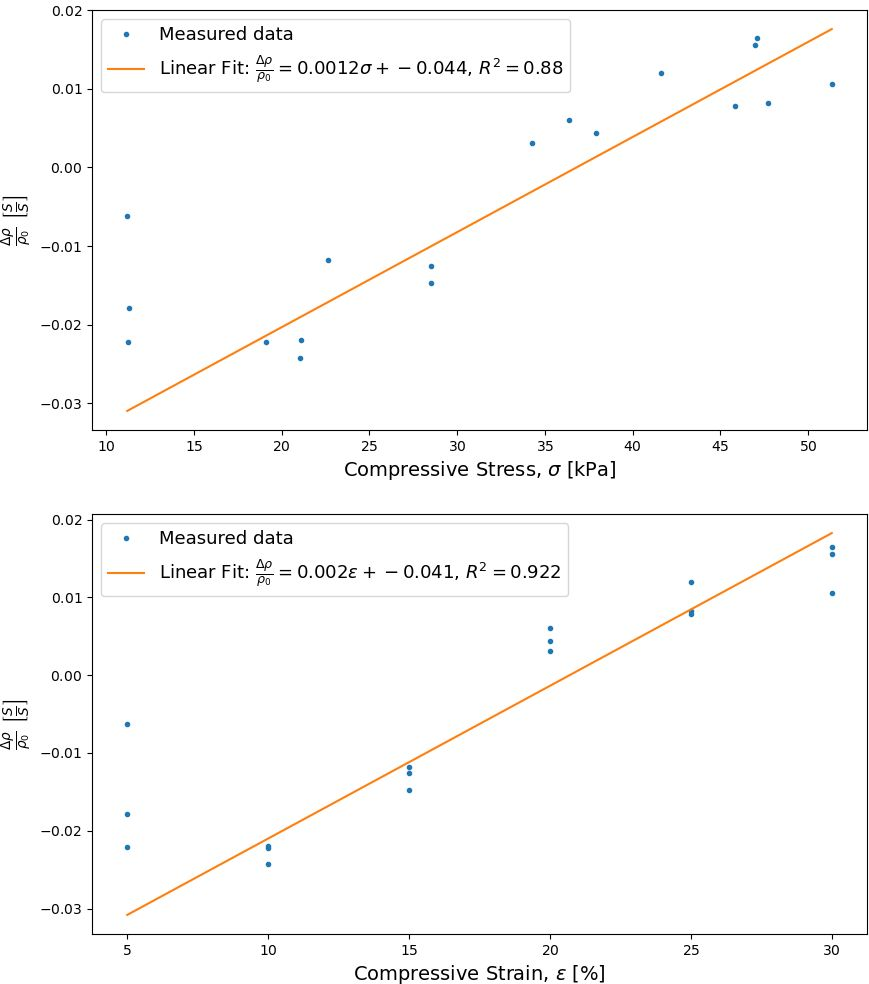
\includegraphics[width=7cm]{Figures/CBSR_9p_cond_stress_strain_sin_titulo.jpg}
%     \caption{Conductance change vs stress (top) and strain (bottom) data and fitted curves for 9 wt\% CBSR. The 5\% strain values ignored as the $\mathrm{std}$ were larger than the conductance change values.}
%     % TODO?: Change Linear fit to 10^{-1} from 10^{-3}
%     \label{fig:quasi_r_9p}
% \end{figure}
% TODO: change plot title

\subsubsection{Transient Piezoresistivity}\label{sec:Transient Piezoresistivity2}
The transient piezoresistive effects observed within a PNEC limit the frequency response of the sensor. An example of the transient response of the material to a repeated compressive strain pulse input is displayed in Figure \ref{fig:stress_seq}, clearly showing the stress relaxation of the material due to its viscoelasticity. 
\begin{figure}[H]
    \centering
    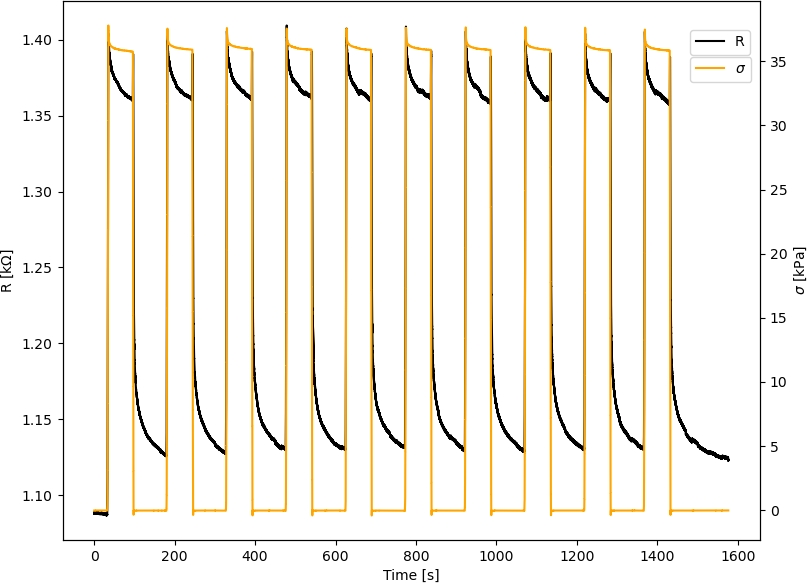
\includegraphics[width=0.7\linewidth]{Figures/CBSR 8 wt 25p strain - 1D test stress seq.jpg}
    \caption{Compressive loading applied to the CBSR 8 wt\% DUT for 10 loading events of 25\% strain.}
    \label{fig:stress_seq}
\end{figure}
In Figure \ref{fig:load_relax_eg} a loading event is shown with the related stress and resistance relaxation curves. The unloading event similarly has a relaxation period for both stress and resistance in the loading case. Unlike the loading stress transient, the resistance transient has a spike during the unloading relaxation event seen in Figure \ref{fig:load_relax_eg}. This rising edge and peak of this spike are ignored and the resistance relaxation edge is characterised.  
\begin{figure}[H]
    \centering
    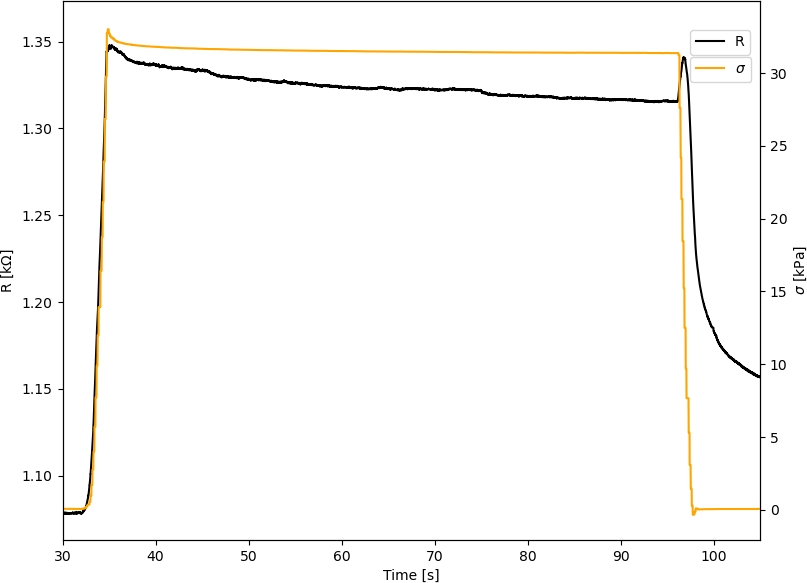
\includegraphics[width=0.7\linewidth]{Figures/CBSR 8 wt 25p strain - 1D stress load unload.jpg}
    \caption{Compressive loading and unloading transients for CBSR 8 wt\% material undergoing a 20\% strain pulse from the first pulse given in Figure \ref{fig:stress_seq}.}
    \label{fig:load_relax_eg}
\end{figure}
For each stress relaxation Equation \ref{eqn:kelvin_general_n2} was fitted to the data. Due to the similarity of  the viscoelastic behaviour seen in the stress-strain relationship, analogously the same generalised linear model was fitted to the resistive relaxation events observed similar to the tensile testing shown in the previous chapter.
\begin{figure}[H]
    \centering
    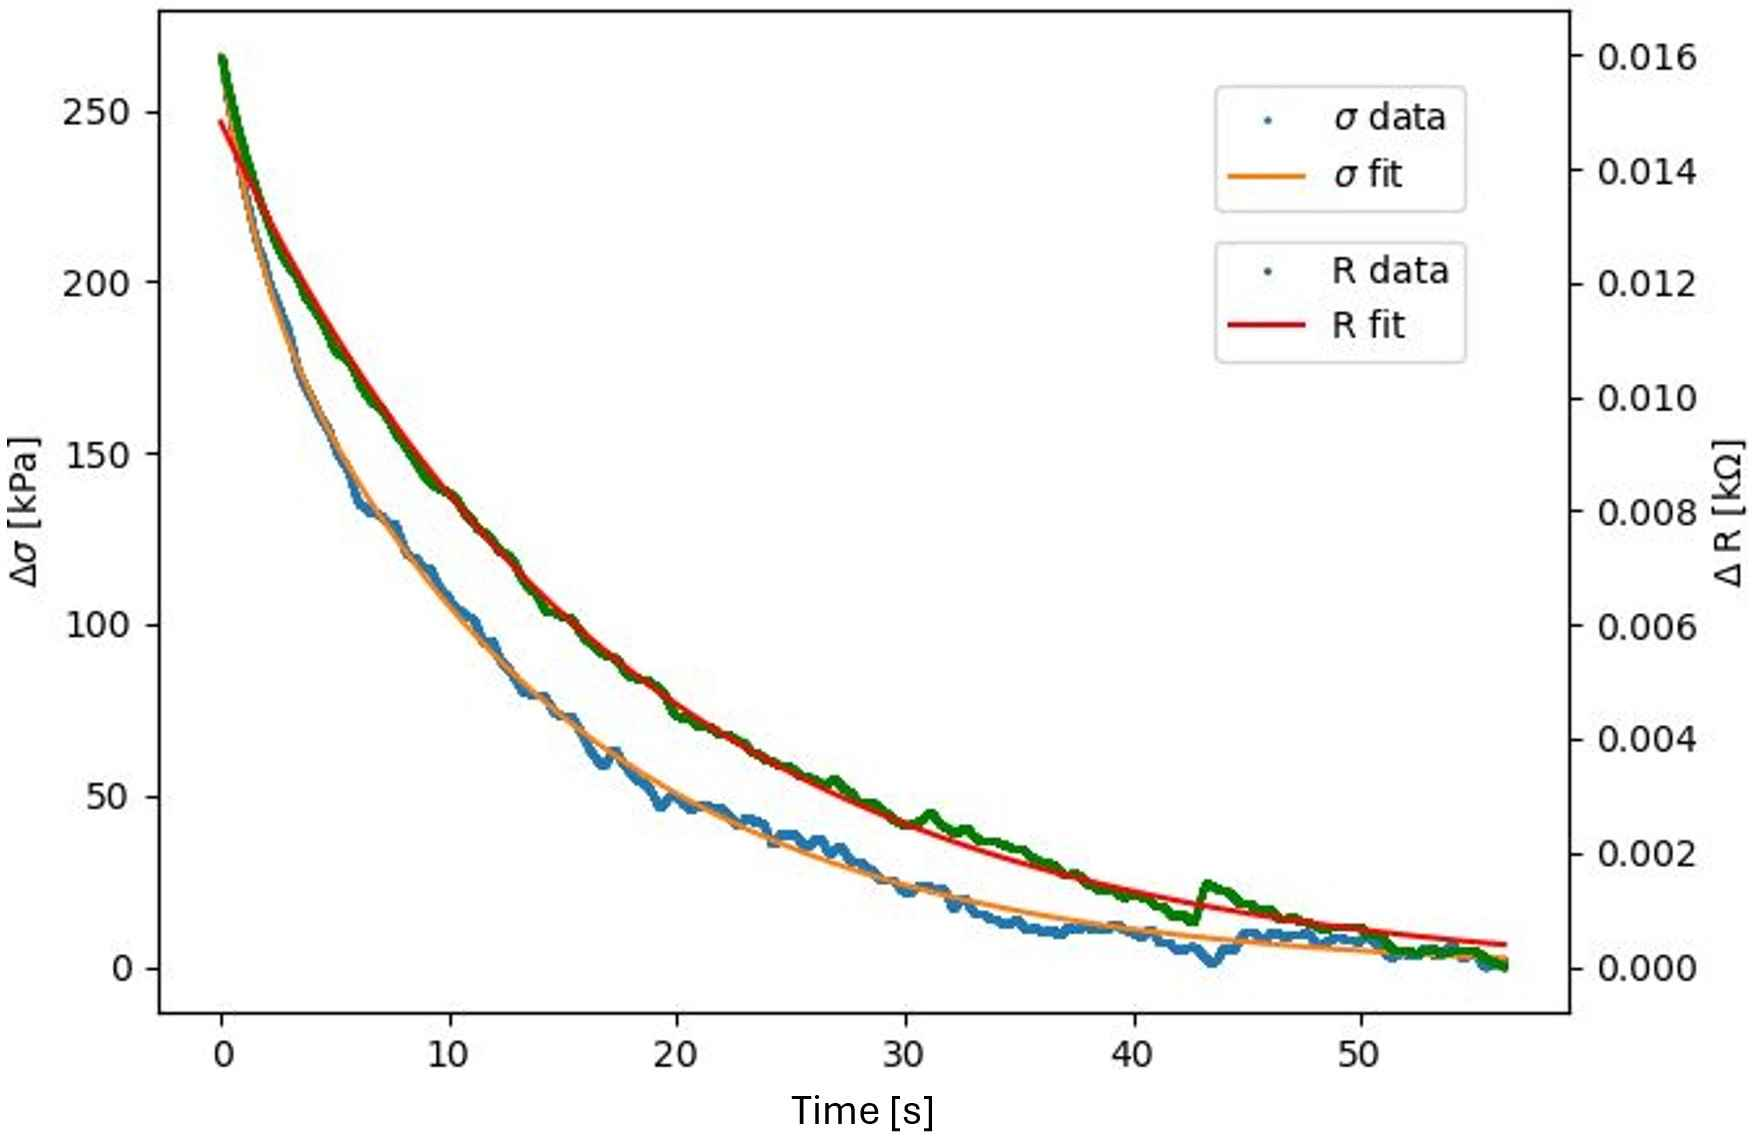
\includegraphics[width=0.7\linewidth]{Figures/Push event 3 - CBSR 8 wt 5p strain - 1D compression test.jpg}
    \caption{The fourth 1D load event, $L_{3}$ on the CBSR 8 wt\% sample using 5\% strain showing a stress, $\sigma$ and resistance, R, relaxation event and their corresponding fitted curves.}
    \label{fig:push_event_relax_example}
\end{figure}
The fitted parameters were found for both 8 and 9 wt\% CBSR samples, giving an indication of the differences due to CB weight percentage and the apparent viscoelasticity.

The settling times of the resistance relaxations give an indication of the frequency response of material. Thus, parameters were fitted to a series of relaxations using Equation \ref{eqn:kelvin_general_n2}, then a series of fit parameters could be used to determine a mean fit. The mean fit was then used to determine the mean settling time over each ten loading events and each of the six strain values. The mean relaxation settling times were compared for each CB weight percentage as shown in Appendices \ref{fig:strain_ts_8p_1D} and \ref{fig:strain_ts_9p_1D}.

% \subsubsection{Sensor System}\label{sec:Sensor System2}
% % TODO:

% \subsubsection{EIT Solver}\label{sec:EIT Inverse Solver2}
% % TODO:


\subsection{Sensor Performance Metrics}\label{sec:Sensor Performance Metrics2}
To validate this 2D pressure sensing platform for specific applications the limits of the sensor must be known. Metrics to analyse and quantify the sensor limits such as noise, spatial-, temporal-, and stress- performance metrics are given in this section.

% \subsubsection{Noise Figure}\label{sec:Noise Figure2}
% To determine whether the noise floor of the material in steady-state was sufficiently low the noise figure was calculated for the unloaded state of the material and given in Table \ref{tab:DUT_nf_char}. 
% % TODO?: Make a table of the average noise figure vs strain vs wt%
% % TODO?: Compare average noise figure and location of load (i.e. are there areas with higher NF values! i.e. where the stress resolution may be lower?)
% % TODO?: Determine why the NF is so high? It's showing that the input noise is damped by EIT??
% \begin{table}[H]
% \caption{DUT noise figure at steady-state}
% \label{tab:DUT_nf_char}
% \begin{center}
% \begin{tabular}{lll}
% \hline
% \textbf{CB wt\%} & $\mathrm{\mu}$\textbf{(NF)} & $\mathrm{std}$\textbf{(NF)}     \\ \hline
% 8           & 1.200    &    0.171               \\
% 9           & 1.146    &    0.112               \\ 
% \hline
% \end{tabular}
% \end{center}
% \end{table}
% It was also observed that the mean NF generally increased as the strain signal increased as shown in \ref{fig:NF_strain_time}.
% \begin{figure}[H]
%     \centering
%     \includegraphics[width=8.5cm]{Figures/CBSR_8p_1_9push_XXstrain_60s_NF_vs_strain_all.jpg}
%     \caption{Noise figure over time for each different strain experiment for CBSR 8 wt\%.}
%     \label{fig:NF_strain_time}
% \end{figure}
% TODO?: Quantify background noise during and between push events from 'ringing' as seen in -> \citep{Russo2017}. Could limit the stress sensor in terms of simultaneous and concurrent pushes.

\subsubsection{Pre-processing}\label{Pre-processing2}
The noise floor limits the detection of small forces. First the noise floor was found from the no load steady-state of material. The maximum noise from the first eight frames was found and this maximum was subtracted from all contiguous images in the time series experiment.
% \begin{figure*}[H]
%     \centering
%     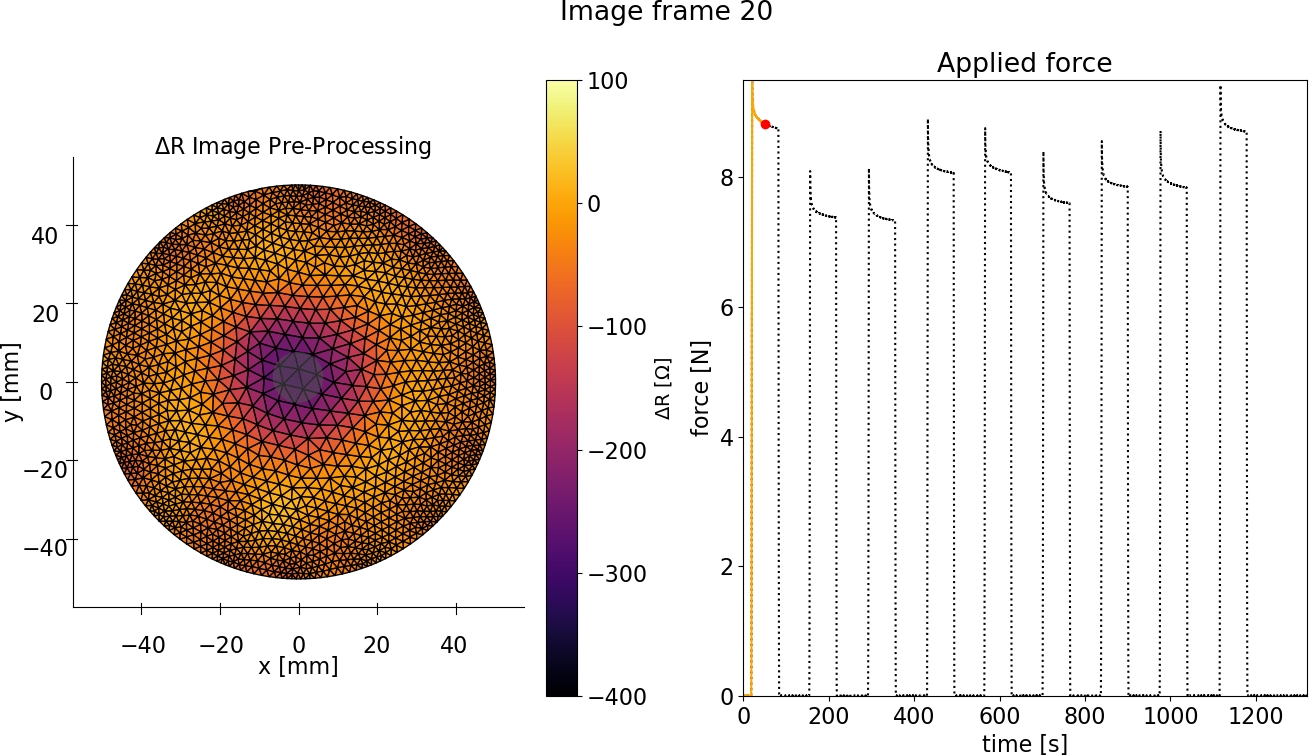
\includegraphics[width=0.8\textwidth]{Figures/CBSR_8p_9push_20strain_60s_4_frame20_pre_processing.jpg}
%     \caption{Left: An example of an unprocessed image from an image reconstruction during a 20\% loading event in the middle of the 8wt\% CBSR domain, shown by the transparent white circle. Right: A force plot with a red dot showing the current force reading for the same image reconstruction frame .}
%     \label{fig:pre_process}
% \end{figure*}

After a noise mask has eliminated the steady state noise floor, different percentage thresholds can be used to compensate for different regularisation and different material push area edge softness as shown in Figure \ref{fig:thresh_masks}.
% \begin{figure}[H]
%     \centering
%     \includegraphics[width=9.3cm]{Figures/CBSR_8p_9push_20strain_60s_4_frame20_all_masks.jpg}
%     \caption{A series of threshold percentage masks 25, 50, 75, 85\% for the same reconstruction given in Figure \ref{fig:noise_floor_mask_8p}}
%     \label{fig:thresh_masks}
% \end{figure}
\begin{figure}[H]
\centering
    \begin{minipage}[t]{.3\textwidth}
        \vspace{0pt}
        \subfloat[][]{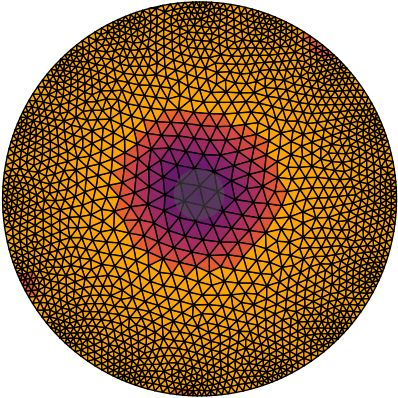
\includegraphics[width=\textwidth]{Figures/CBSR_8p_9push_20strain_60s_4_frame20_25p_mask_cropx2.jpg}\label{thresh25}}
        \vfill
        \subfloat[][]{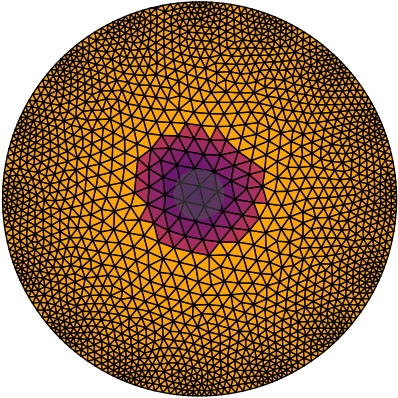
\includegraphics[width=\textwidth]{Figures/CBSR_8p_9push_20strain_60s_4_frame20_50p_mask_cropx2.jpg}\label{thresh50}}
        \vspace{0pt}
    \end{minipage}%
    \hspace{0.05\linewidth}
    \begin{minipage}[t]{.3\textwidth}
        \vspace{0pt}
        \subfloat[][]{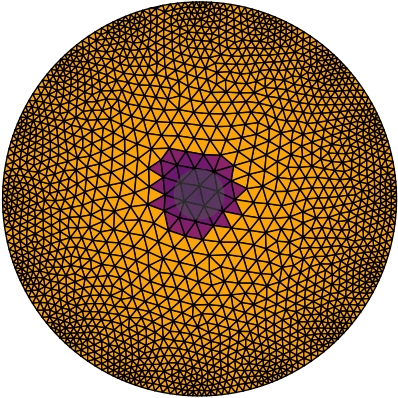
\includegraphics[width=\textwidth]{Figures/CBSR_8p_9push_20strain_60s_4_frame20_75p_mask_cropx2.jpg}\label{thresh75}}
        \vfill
        \subfloat[][]{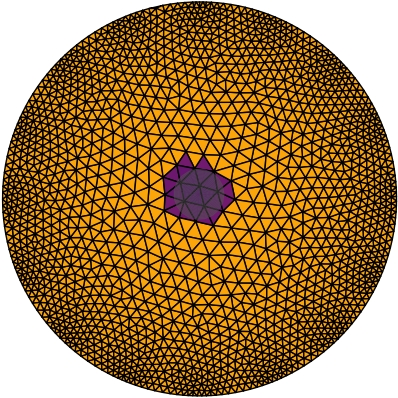
\includegraphics[width=\textwidth]{Figures/CBSR_8p_9push_20strain_60s_4_frame20_85p_mask_cropx2.jpg}\label{thresh85}}
        \hfill
    \end{minipage}
    \hspace{0.05\linewidth}
    \begin{minipage}[t]{.1\textwidth}
        \vspace{1cm}
        \subfloat[][]{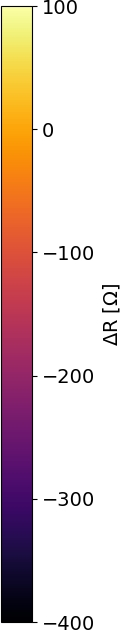
\includegraphics[width=\textwidth]{Figures/CBSR_8p_9push_20strain_60s_4_frame20_scale_bar.jpg}\label{colour_bar}}
        \hfill
    \end{minipage}  
\caption{A series of threshold percentage masks (A) 25\%, (B) 50\%, (C) 75, and (D) 85\% for the same reconstruction given in Figure \ref{fig:noise_floor_mask_8p}. (E) is the resistance change scale bar.}
\label{fig:thresh_masks}
\end{figure}
The threshold masked image blobs and the force applicator shapes in Figures \ref{thresh25} - \ref{thresh85} are compared and quantified in the following section.

\subsubsection{Spatial Performance}\label{sec:Spatial Performance2}
%% TODO: Turn this section into a flowing story - Pre-processing highlights points of interest. Prove good data is being captured, i.e. E_CoM is super low, SD is low and A_OL is high!.
To properly determine where the area and perimeter of a load are, multiple threshold mask filters were applied. To validate the threshold mask percentages
 the three main performance characteristics were displayed as separate time series for each material, each applied strain, and each threshold percentage mask. These time series show how each metric changed over the course of a loading test sequence and how the metrics vary across the surface of the DUT. An example comparing this time series data for two instances where a 20\% strain pulse train was applied to a the nine loading locations with multiple threshold mask percentages is shown in Figures \ref{fig:recon_perform_8p} and Appendix \ref{fig:recon_perform_9p} for for 8 and 9 wt\% CBSR samples respectively.
% TODO: Table of threshold percentages (25, 50, 75, 85\%) comparing the mean of the 3 performance metrics for 8 and/or 9 wt\%
    
\begin{figure}[H]
    \centering
    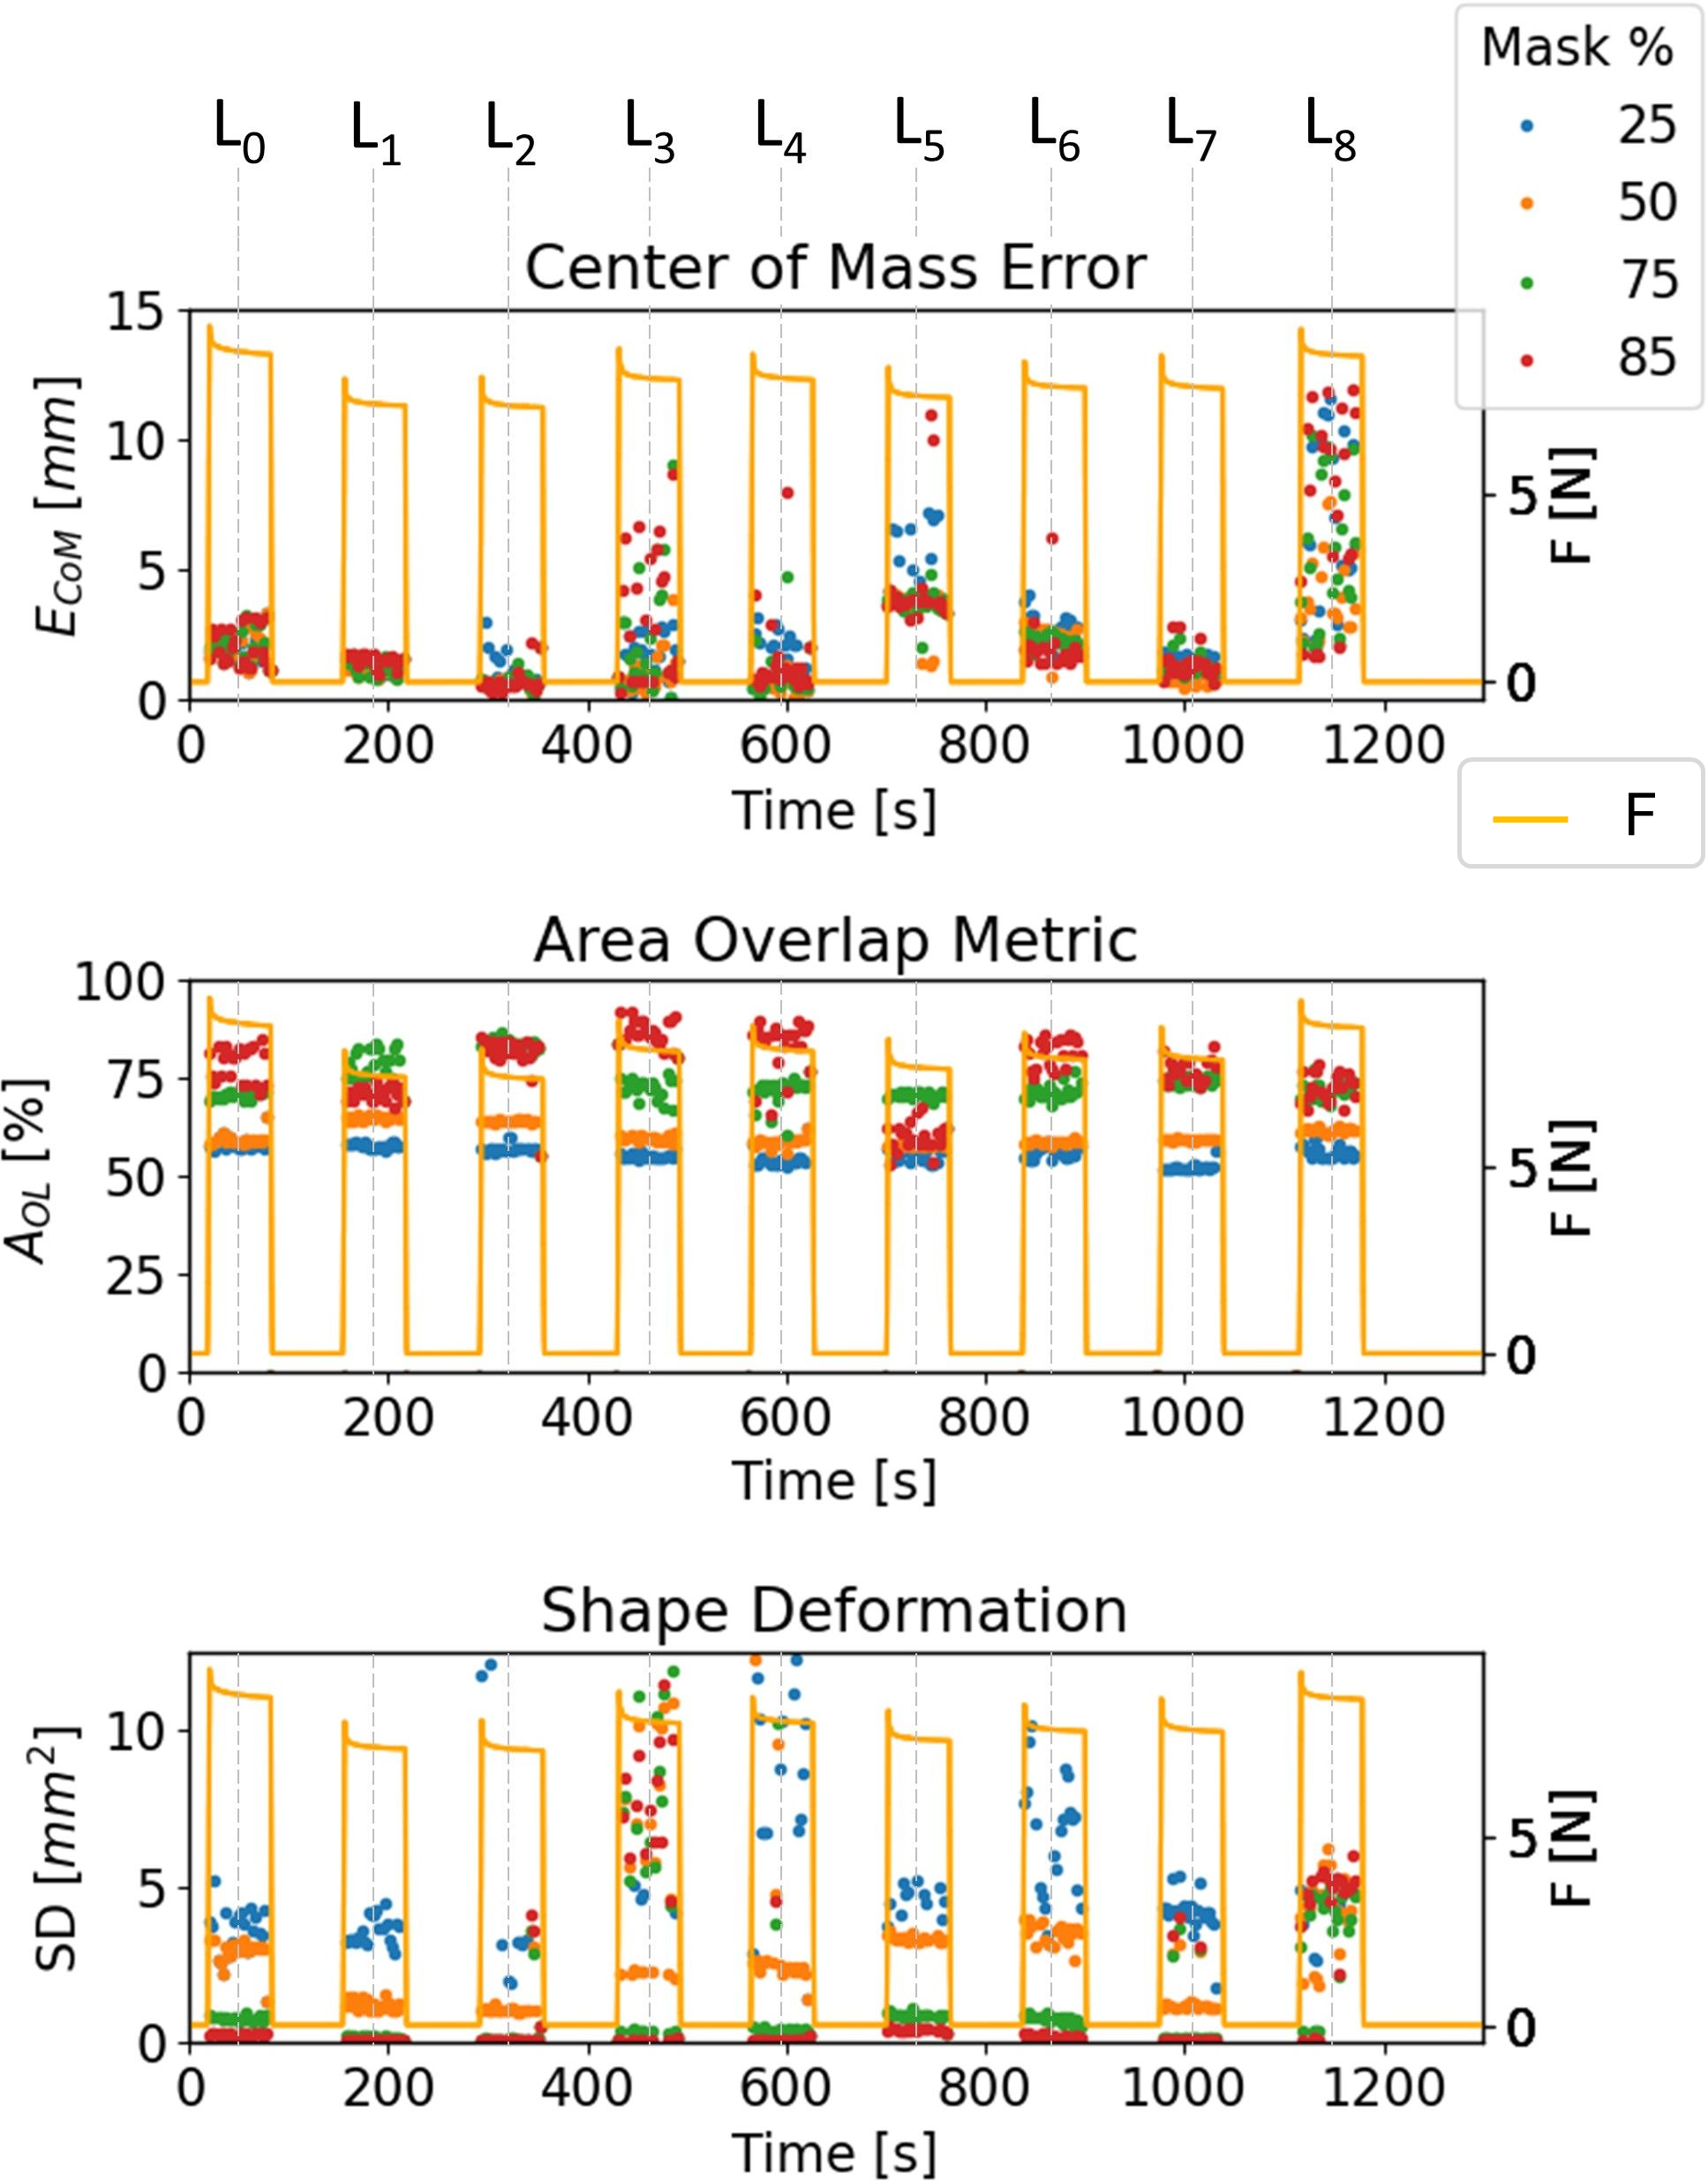
\includegraphics[width=0.8\linewidth]{Figures/CBSR_8p_9push_20strain_60s_4_metrics_thresh_masks_v2_numbd_F.png}
    \caption{Spatial performance metrics comparing threshold percentages of 25, 50, 75, and 85\% for a 8 wt\% CBSR sample being loaded with 20\% compressive strain in nine areas, $L_{0-8}$, shown in Figure \ref{fig:force_app_map}.} % TODO?: Determine better way of displaying these metrics??
    \label{fig:recon_perform_8p}
\end{figure}
% \begin{figure}[H]
%     \centering
%     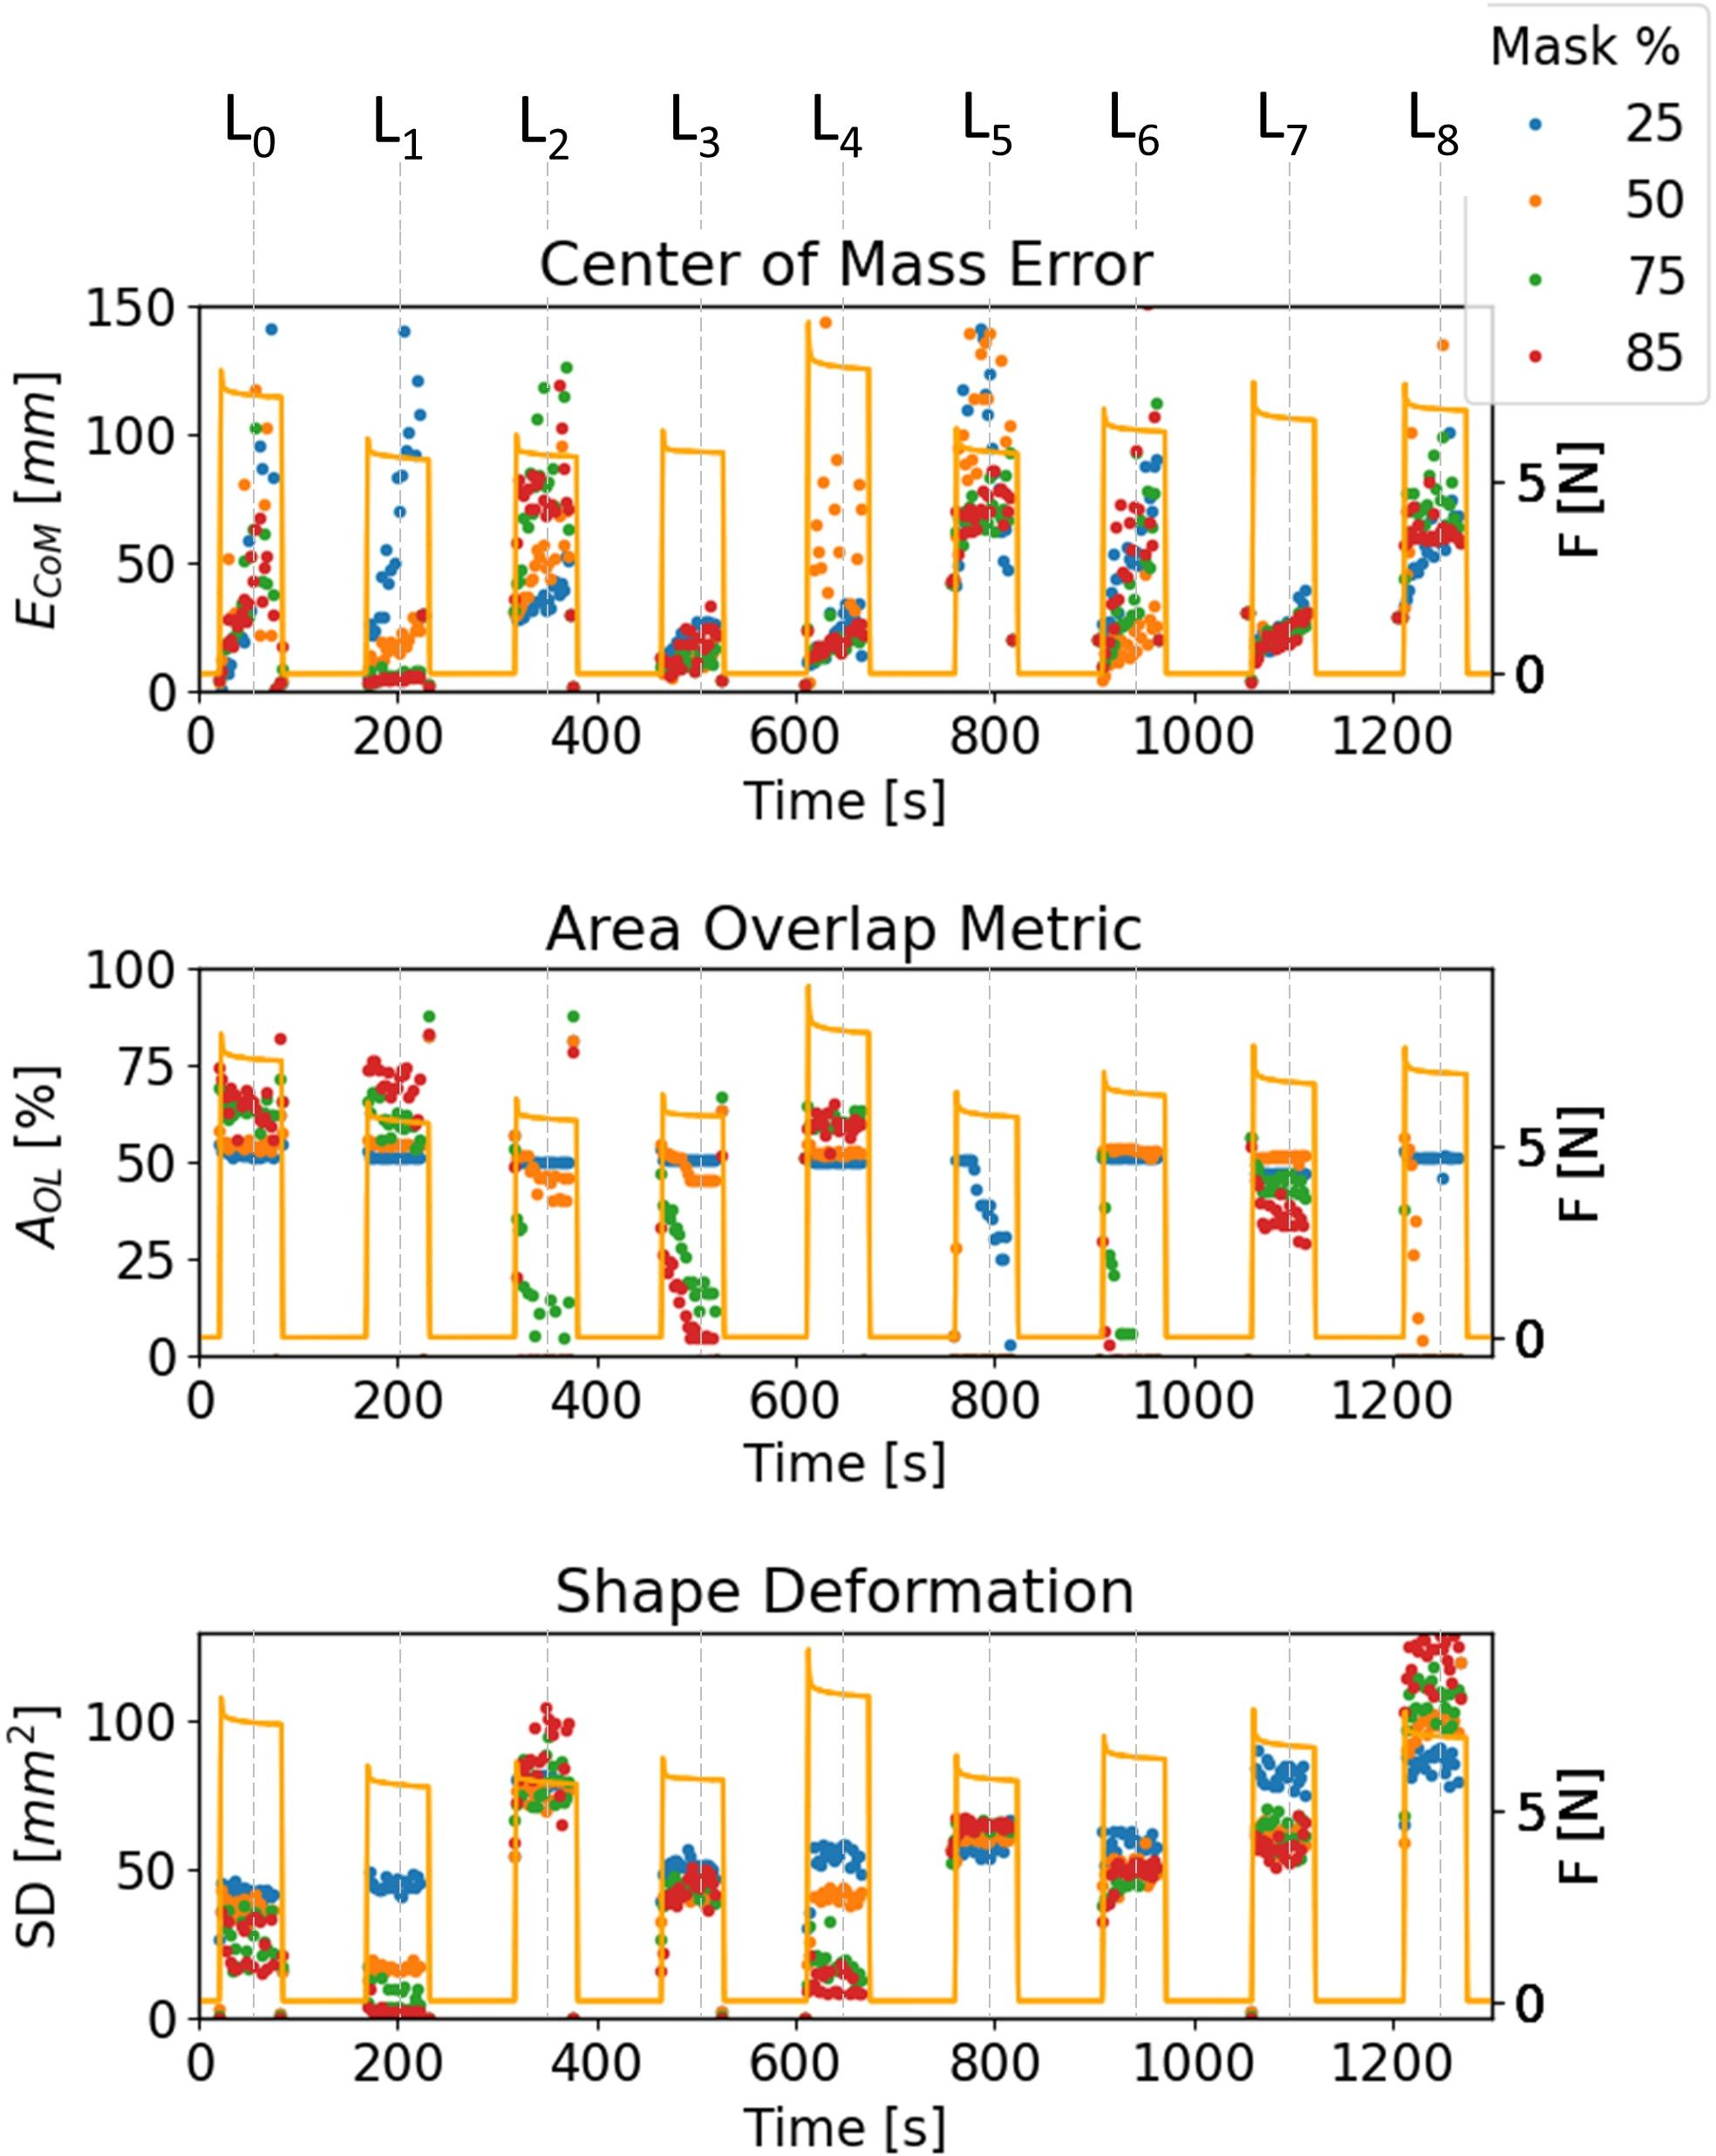
\includegraphics[width=8.3cm]{Figures/CBSR_9p_9push_20strain_60s_4_metrics_thresh_masks_v2_numbd.jpg}
%     \caption{Spatial performance metrics comparing threshold percentages of 25, 50, 75, and 85\% for 9 wt\% CBSR sample being loaded with 20\% compressive strain in nine areas, $L_{0-8}$, shown in Fig \ref{fig:force_app_map}.} % TODO?: Determine better way of displaying these metrics??
%     \label{fig:recon_perform_9p}
% \end{figure}

% TODO: Somehow show the how the blob_metrics change for % threshold and change for % strain.
    % Could plot blob_metric_loadings vs %'s (i.e. 9 load curves overlapped) 

The percentage threshold masks from 25 - 85\% were compared by finding the mean of all of the spatial performance metrics for each strain from 5 - 30\%. The mean and standard deviation for each of these metrics from the data shown in Figure \ref{fig:recon_perform_8p} is given in Tables \ref{tab:spatial_metrics_stats_8p_strain20} and \ref{tab:spatial_metrics_stats_8p_strain20_loads}.

\begin{table}[H]
    \caption{CBSR 8 wt\% mean and standard deviation for spatial performance metrics across of a nine loads, $L_0$-$L_8$ and strain value 20\%.}
    \label{tab:spatial_metrics_stats_8p_strain20}
    \centering
    \begin{tabular}{p{0.7cm}p{2cm}p{2.1cm}p{1.8cm}}
    \hline
        \% thresh & $E_{CoM}$ [mm] & $A_{OL}$ [\%] & $S\!D$ [mm$^2$]\\ \hline
        0.25& 4.1 $\pm$ 6.3& 53.3 $\pm$ 15.3& 10.4 $\pm$ 9.3 \\
        0.5& 3.3 $\pm$ 6.3& 57.5 $\pm$ 16.3& 3.6 $\pm$ 4.4 \\
        0.75& 3.8 $\pm$ 6.3& 69.6 $\pm$ 19.8& 2.4 $\pm$ 5.8 \\
        0.85& 4.1 $\pm$ 6.4& 72.5 $\pm$ 21.7& 2.4 $\pm$ 6.5 \\
        \hline
    \end{tabular}
\end{table}

\begin{table}[H]
    \caption{CBSR 8 wt\% mean and standard deviation for spatial performance metrics of nine loads, $L_0$-$L_8$, a 85\% percentage threshold mask, and strain value 20\%.}
    \label{tab:spatial_metrics_stats_8p_strain20_loads}
    \centering
    \begin{tabular}{p{0.7cm}p{2cm}p{2.1cm}p{2.1cm}}
        \hline       
        Load & $E_{CoM}$ [mm] & $A_{OL}$ [\%] & $S\!D$ [mm$^2$]\\ \hline
        $L_0$ & 2.05 $\pm$ 0.70& 80.39 $\pm$ 4.19& 0.28 $\pm$ 0.01\\
        $L_1$& 1.53 $\pm$ 0.23& 72.32 $\pm$ 1.74& 0.12 $\pm$ 0.01\\
        $L_2$& 0.67 $\pm$ 0.41& 83.00 $\pm$ 2.38& 0.48 $\pm$ 1.16\\
        $L_3$& 3.29 $\pm$ 2.17& 87.93 $\pm$ 2.68& 5.25 $\pm$ 3.78\\
        $L_4$& 1.44 $\pm$ 1.61& 84.81 $\pm$ 5.78& 2.76 $\pm$ 5.65\\
        $L_5$& 4.43 $\pm$ 2.09& 61.08 $\pm$ 3.29& 7.39 $\pm$ 16.31\\
        $L_6$& 2.03 $\pm$ 1.05& 82.19 $\pm$ 3.55& 3.14 $\pm$ 8.57\\
        $L_7$& 1.49 $\pm$ 0.56& 77.68 $\pm$ 2.46& 0.66 $\pm$ 1.25\\
        $L_8$& 6.95 $\pm$ 3.67& 73.69 $\pm$ 3.60& 3.78 $\pm$ 2.01\\
        \hline
    \end{tabular}
\end{table}

% \begin{table}[H]
%     \caption{CBSR 8 wt\% mean and standard deviation for spatial performance metrics over of a nine loads, $L_0$-$L_8$ and six strain values (5 - 30\%).}
%     \label{tab:spatial_metrics_stats_8p}
%     \centering
%     \begin{tabular}{p{0.7cm}p{2cm}p{1.8cm}p{1.8cm}}
%     \hline
%         \% thresh & $E_{CoM}$ [mm] & $A_{OL}$ [\%] & $S\!D$ [mm$^2$]\\ \hline
%         25 & \textbf{25.68} $\pm$ 29.91 & 42.29 $\pm$ 12.88 & 44.10 $\pm$ 16.64 \\
%         50 & 79.29 $\pm$ 207.25 & 39.27 $\pm$ 12.80 & 41.26 $\pm$ 16.60 \\
%         75 & 141.12 $\pm$ 519.81 & 37.42 $\pm$ 13.67 & 37.89 $\pm$ 16.28 \\
%         85 & 52.10 $\pm$ 68.97 & 36.26 $\pm$ 13.72 & \textbf{37.62} $\pm$ 16.60 \\
%         \hline
%     \end{tabular}
% \end{table}
% \begin{table}[H]
%     \caption{CBSR 9 wt\% mean and standard deviation for spatial performance metrics over of a nine loads, $L_0$-$L_8$ and six strain values (5 - 30\%).}
%     \label{tab:spatial_metrics_stats_9p}
%     \centering
%     \begin{tabular}{p{0.7cm}p{2cm}p{1.8cm}p{1.8cm}}
%     \hline
%         \% thresh & $E_{CoM}$ [mm] & $A_{OL}$ [\%] & $S\!D$ [mm$^2$]\\ \hline
%         25 & 102.11 $\pm$ 233.19 & 45.90 $\pm$ 12.95 & 59.58 $\pm$ 10.72 \\
%         50 & 194.97 $\pm$ 550.06 & 40.92 $\pm$ 13.50 & 54.07 $\pm$ 9.92 \\
%         75 & 60.43 $\pm$ 74.23 & 33.55 $\pm$ 14.11 & 49.71 $\pm$ 10.88 \\
%         85 & \textbf{53.78} $\pm$ 54.16 & 30.08 $\pm$ 13.87 & \textbf{49.18} $\pm$ 11.44 \\ \hline
%         \hline
%     \end{tabular}
% \end{table}
%%%% ALT table format %%%%
% \begin{table}[H]
%     \caption{CBSR 8 wt\% mean and standard deviation for spatial performance metrics over of a nine loads, $L_0$-$L_8$ and six strain values (5 - 30\%).}
%     \label{tab:spatial_metrics_stats_8p}
%     \centering
%     \begin{tabular}{p{.65cm}p{.85cm}p{.85cm}p{.75cm}p{.75cm}p{.75cm}p{.75cm}}
%     \hline
%         \% thresh & $\mu_{CoM}$ [mm] & $\mathrm{std}_{CoM}$ [mm]& $\mu_{A_{OL}}$ [\%] & $\mathrm{std}_{A_{OL}}$ [\%] & $\mu_{S\!D}$ [mm$^2$]& $\mathrm{std}_{SD}$ [mm$^2$]\\ \hline
%         25 & \textbf{25.68} & 29.91 & 42.29 & 12.88 & 44.10 & 16.64 \\
%         50 & 79.29 & 207.25 & 39.27 & 12.80 & 41.26 & 16.60 \\
%         75 & 141.12 & 519.81 & 37.42 & 13.67 & 37.89 & 16.28 \\
%         85 & 52.10 & 68.97 & 36.26 & 13.72 & \textbf{37.62} & 16.60 \\
%         \hline
%     \end{tabular}
% \end{table}
% \begin{table}[H]
%     \caption{CBSR 9 wt\% mean, $\mu$, and standard deviation, $std$, of spatial performance metrics}
%     \label{tab:spatial_metrics_stats_9p}
%     \centering
%     \begin{tabular}{p{.65cm}p{.85cm}p{.85cm}p{.75cm}p{.75cm}p{.75cm}p{.75cm}}
%     \hline
%         \% thresh & $\mu_{CoM}$ [mm] & $\mathrm{std}_{CoM}$ [mm]& $\mu_{A_{OL}}$ [\%] & $\mathrm{std}_{A_{OL}}$ [\%] & $\mu_{S\!D}$ [mm$^2$]& $\mathrm{std}_{SD}$ [mm$^2$]\\ \hline
%         25 & 102.11 & 233.19 & 45.90 & 12.95 & 59.58 & 10.72 \\
%         50 & 194.97 & 550.06 & 40.92 & 13.50 & 54.07 & 9.92 \\
%         75 & 60.43 & 74.23 & 33.55 & 14.11 & 49.71 & 10.88 \\
%         85 & \textbf{53.78} & 54.16 & 30.08 & 13.87 & \textbf{49.18} & 11.44 \\ \hline
%     \end{tabular}
% \end{table}
%%%% ALT table format %%%%

% TODO: Redo these results using threshold masking and blob separation to see if better results can be obtained. CoM error of 25.68 and 53.78 is a bit shit!??

% TODO?: Create an absolute threshold mask using known expected limits of material in 1D. (i.e. expected dR/R_0=4% for a strain=5% for CBSR 8%)
% TODO?: Compare threshold masking 50-85% with absolute threshold masking?
% TODO?: Place performance metric plots in the appendices?

\subsection{Randomised Location and Strain Testing}
In a real world application the sensor platform in this work will likely experience a large range of unknown loads in various locations. To ensure that the device operates in a similar fashion to that seen in the structured experimental data, a randomised experiment was completed. The randomised experiment loads were at ten randomised radii, $r_{rand}$, angles, $\theta_{rand}$, and strain values, all within the ranges, 0 - 40\% of the domain radius, 0 - 360$\degree$, and  5 - 30\% respectively.

\begin{figure}[H]
    \centering
    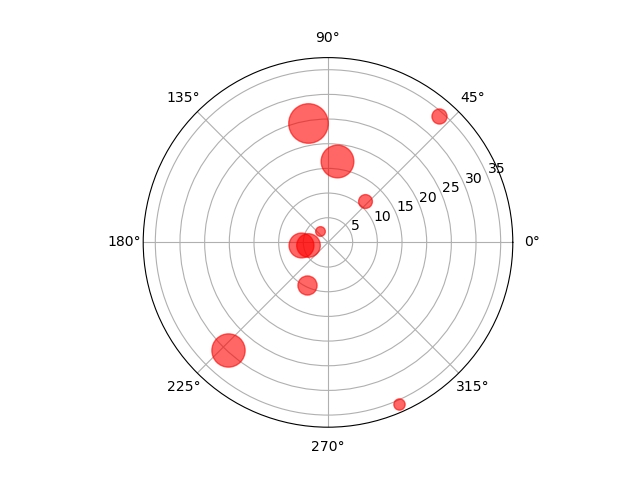
\includegraphics[width=0.7\linewidth]{Figures/rand1_strain_aplc_points.jpg}
    \caption{The ten random load point locations, $L_{rand}$, and random strain values proportional to red circle size as shown on a polar plot.}
    \label{fig:rand1_load_locs}
\end{figure}

Spatial performance metrics for these tests are given in Tables \ref{tab:spatial_ecom_metrics_stats_8p_rand_loads} and \ref{tab:spatial_sd_metrics_stats_8p_rand_loads} with the load points and their magnitudes shown diagrammatically in Figure \ref{fig:rand1_load_locs}. A pseudo-random number generator with a uniform distribution was used for all randomly generated data.

% Random loc/strain values used >>
% r = [5.42743849862509, 29.846456136299985, 4.181660082237304, 34.04603730123931, 35.80371089244604, 9.55811959727824, 2.769985486438258, 11.156805670844921, 24.567831277259092, 16.589765149647803]
% theta = [9.538757518092709, 336.97294194577626, 317.4390882463128, 69.96700648150347, 137.07095150991276, 54.52712421011869, 259.78313980093276, 113.93715998989623, 240.50066010959594, 252.79291781930928]
% strain = [17.94306607, 23.95295652, 16.99213858, 10.88333719,  8.1215735, 13.80547079,  7.00766015,  9.95756214, 28.47087393, 23.59077957]
% (x,y) push_points = [[[-5.392221801367152, -0.6172784632712794], [-20.306653778948643, -21.8735172342719],
                % [-4.141772916377541, -0.576192808475054], [22.419426953903425, 25.622294022510296], 
                % [14.326545277267826, -32.812433833659064], [-4.163882510295342, -8.60347212910758], 
                % [-1.568040444519299, 2.283433546094633], [7.448211278155931, 8.306531257567638], 
                % [-4.127919477779628, 24.218559297630353], [1.743523889492196, 16.497891749167188]]] 

% ::: Random sequence #1 gathered for 8/9 wt% :::
% CBSR_8p_OG_10push_RAND1_strain_120s_1mA_3:
% ----------------MEANS------------------
% E_com L_0 mean = 3.09 +/- 0.68 mm (+\- 22.00%)
% E_com L_1 mean = 1.89 +/- 0.39 mm (+\- 20.84%)
% E_com L_2 mean = 7.85 +/- 2.26 mm (+\- 28.83%)
% E_com L_3 mean = 6.03 +/- 3.54 mm (+\- 58.77%)
% E_com L_4 mean = 13.87 +/- 0.58 mm (+\- 4.20%)
% E_com L_5 mean = 6.03 +/- 1.01 mm (+\- 16.72%)
% E_com L_6 mean = 12.01 +/- 8.12 mm (+\- 67.64%)
% E_com L_7 mean = 5.07 +/- 1.19 mm (+\- 23.52%)
% E_com L_8 mean = 2.33 +/- 0.15 mm (+\- 6.27%)
% E_com L_9 mean = 3.09 +/- 0.43 mm (+\- 13.98%)
% ---------------------------------------
% E_com total mean = 6.13 +/- 1.84 mm (+\- 26.28%)
% ---------------------------------------
% CBSR_9p_2_10push_RAND1_strain_120s_1mA_2:
% ----------------MEANS------------------
% E_com L_0 mean = 3.06 +/- 0.54 mm (+\- 17.73%)
% E_com L_1 mean = 5.00 +/- 0.60 mm (+\- 12.09%)
% E_com L_2 mean = 9.01 +/- 0.95 mm (+\- 10.52%)
% E_com L_3 mean = 2.86 +/- 0.45 mm (+\- 15.79%)
% E_com L_4 mean = 7.69 +/- 4.58 mm (+\- 59.51%)
% E_com L_5 mean = 10.29 +/- 4.44 mm (+\- 43.17%)
% E_com L_6 mean = 28.73 +/- 10.89 mm (+\- 37.93%)
% E_com L_7 mean = 12.04 +/- 1.90 mm (+\- 15.78%)
% E_com L_8 mean = 2.43 +/- 0.17 mm (+\- 6.86%)
% E_com L_9 mean = 7.07 +/- 0.45 mm (+\- 6.35%)
% ---------------------------------------
% E_com total mean = 8.82 +/- 2.50 mm (+\- 22.57%)
% ---------------------------------------
\begin{table}[H]
    \caption{CBSR 8 and 9 wt\% mean and standard deviation for $E_{CoM}$ spatial performance metrics of ten random locations, $L_{rand}$ and random strains $\varepsilon$}. % TODO: complete these tests with best blob algorithm??
    \label{tab:spatial_ecom_metrics_stats_8p_rand_loads}
    \centering
    \begin{tabular}{p{2.6cm}p{1.0cm}p{2.0cm}p{2.0cm}}
        \hline       
        $L_{rand}$(r, $\theta$) [mm, $\degree$] & $\varepsilon$ [\%] & 8wt\% $E_{CoM}$ [mm] & 9wt\% $E_{CoM}$ [mm] \\ \hline
        (5.4, 10) & 17.9 & 3.1 $\pm$ 0.7 & 3.1 $\pm$ 0.5 \\
        (29.8, 337) & 24.0 & 1.9 $\pm$ 0.4 & 5.0 $\pm$ 0.6 \\
        (4.2, 317) & 17.0 & 7.9 $\pm$ 2.2 & 9.0 $\pm$ 1.0 \\
        (34.0, 70) & 10.9 & 6.0 $\pm$ 3.5 & 2.9 $\pm$ 0.5 \\
        (35.8, 137) & 8.1 & 13.9 $\pm$ 0.6 & 7.7 $\pm$ 4.6 \\
        (9.6, 55) & 13.8 & 6.0 $\pm$ 1.0 & 10.3 $\pm$ 4.4 \\
        (2.8, 260) & 7.0 & 12.0 $\pm$ 8.1 & 28.7 $\pm$ 10.9 \\
        (11.2, 114) & 10.0 & 5.1 $\pm$ 1.2 & 12.0 $\pm$ 1.9 \\
        (24.6, 241) & 28.5 & 2.3 $\pm$ 0.2 & 2.4 $\pm$ 0.2 \\
        (16.6, 253) & 23.6 & 3.1 $\pm$ 0.4 & 7.1 $\pm$ 0.5 \\
        \hline
    \end{tabular}
\end{table}

% >>> shape deformation rand1 data >>>>
% CBSR_8p_OG_10push_RAND1_strain_120s_1mA_3:
% SD mean = 28.37019888870724 +/- 36.375087100802475 mm^2
% SD L_0 mean = 10.060360313590907 +/- 0.759300498717798 mm^2
% SD L_1 mean = 62.24669908647688 +/- 1.256008556309175 mm^2
% SD L_2 mean = 18.678952508510964 +/- 5.90188359500409 mm^2
% SD L_3 mean = 20.167032393462872 +/- 4.703254741118465 mm^2
% SD L_4 mean = 124.79406198440728 +/- 2.7668381472395027 mm^2
% SD L_5 mean = 24.778125232068426 +/- 1.8924413328912213 mm^2
% SD L_6 mean = 15.581052535551132 +/- 4.4977276184355635 mm^2
% SD L_7 mean = 4.494701245816866 +/- 0.8615435669853827 mm^2
% SD L_8 mean = 2.6039946424205165 +/- 0.0603816721645818 mm^2
% SD L_9 mean = 0.2970089447665243 +/- 0.05963041986632069 mm^2
% CBSR_9p_2_10push_RAND1_strain_120s_1mA_2:
% SD mean = 21.968395901369384 +/- 24.745674553451416 mm^2
% SD L_0 mean = 9.75014241821507 +/- 0.6037324879071962 mm^2
% SD L_1 mean = 52.83801393266161 +/- 1.2892792396287853 mm^2
% SD L_2 mean = 21.67315757358719 +/- 2.229797920831935 mm^2
% SD L_3 mean = 13.72061775900543 +/- 0.8268867152710873 mm^2
% SD L_4 mean = 81.49754745447942 +/- 13.80657715514137 mm^2
% SD L_5 mean = 19.214266559748953 +/- 1.7843762256318092 mm^2
% SD L_6 mean = 12.720703647888275 +/- 1.0473139441454 mm^2
% SD L_7 mean = 4.571612355574054 +/- 0.6300399075442432 mm^2
% SD L_8 mean = 2.5877212275097996 +/- 0.07453517449567228 mm^2
% SD L_9 mean = 1.1101760850240219 +/- 0.12545983187747647 mm^2

\subsubsection{Temporal Performance}\label{sec:Temporal Performance2}
Temporal performance is crucial for time sensitive applications and the settling time of the sensing material domain must be known to apply a quasi-static force model. The fitted stress and resistance relaxation parameters were found for both 8 and 9 wt\% CBSR samples, giving an indication of the frequency response of material across all experiments. To ensure a good fit all fits with an $R^2$ value less than 0.85 were eliminated, as they were a result of poor data or poor fitting algorithm implementation.

% using the 85\% percentage threshold masked images. 

% TODO: Generate a blob thresholded `Rblob' plot to show resistive relaxation for the blobs seen for :
    % - CBSR 8p
    % - CBSR 9p
    
% \begin{figure}[H]
%     \centering
%     \includegraphics[width=8cm]{Figures/2D Push event 6 - CBSR 9 wt 5p strain - 2D compression test.jpg}
%     \caption{An example plot of the 2D load event number 6 on the CBSR 9 wt\% sample using 5\% strain showing a stress, $\sigma$ and resistance, R, relaxation event and their corresponding fitted curves.}
%     \label{fig:blob_global_relaxation}
% \end{figure}

\begin{figure}[H]
    \centering
    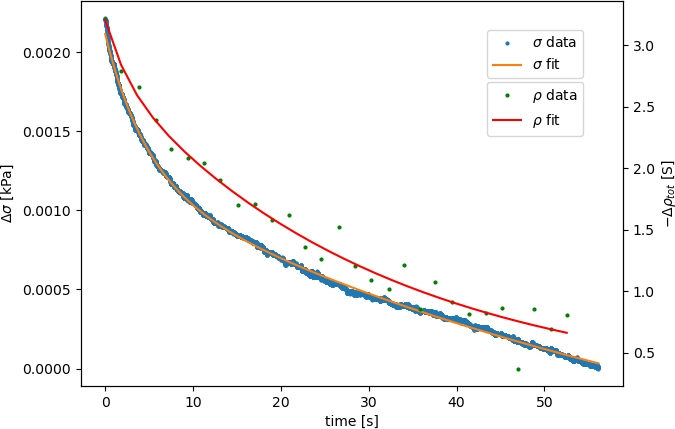
\includegraphics[width=0.7\linewidth]{Figures/2D Push event 0 - CBSR 9 wt 30p strain - 2D compression.jpg}
    \caption{EIT load event $L_0$ on the CBSR 9 wt\% sample using 30\% strain showing a stress, $\sigma$ and conductance, $\rho$, relaxation event and their corresponding fitted curves.}
    \label{fig:blob_global_relaxation}
\end{figure}

The mean settling time for each strain was calculated across relaxations for all strains, all 9 locations, and all 3 trials. The settling times were compared for each CB weight percentage as shown in Appendices \ref{fig:strain_ts_8p} and \ref{fig:strain_ts_9p}.
% \begin{figure}[H]
%     \centering
%     \includegraphics[width=8cm]{Figures/CBSR_8p_1_9push_XXstrain_60s_X_ts_vals_vs_strain_2D_sin_titulo.jpg}
%     \caption{Mean settling time for various strains applied to CBSR 8 wt\% with the error bars showing the standard deviation of each settling time.}
%     \label{fig:strain_ts_8p}
% \end{figure}
% \begin{figure}[H]
%     \centering
%     \includegraphics[width=8cm]{Figures/CBSR_9p_2_9push_XXstrain_60s_1mA_X_ts_vals_vs_strain_2D_sin_titulo.jpg}
%     \caption{Mean settling time for various strains applied to CBSR 9 wt\% with the error bars showing the standard deviation of each settling time.}
%     \label{fig:strain_ts_9p}
% \end{figure}
% TODO: create table of settling time mean and stdev for each strain for:
    % - CBSR 8p
    % - CBSR 9p

\subsubsection{Localise Force Sensing Performance}\label{sec:Localised Force Sensing Performance2}
To determine the localised force sensing performance the linear quasi-static Equation \ref{eqn:quasi_rstress} was applied to the percentage threshold masked image blobs developed in section \ref{sec:Spatial Performance}.

To determine the force sensing limits of the material, the force estimated erroneously due to the EIT reconstruction noise floor was determined. The noise floor is the noise observed over a time series of EIT images when the DUT has zero load applied and there are no resistive transient effects present. The noise floor, $\Delta\rho_n$, of unloaded relaxed 8 and 9 wt\% CBSR DUT conductance images were calculated as $\pm$0.33 and $\pm$0.34 $\mu S$ respectively. An average DUT inter-electrode conductance, $\rho_{int}$, of 55.3 and 222.2 $\mu S$ was derived from Table \ref{tab:DUT_char} for CBSR 8 and 9 wt\% respectively. A relative change of conductance value, $\frac{\Delta\rho_{n}}{\rho_{int}}$, was then calculated as 5.97$\times10^{-3}$ and 1.53$\times10^{-3}$ $\mu S$ for CBSR 8 and 9 wt\% respectively. From the quasi-static piezoresistivity Equation \ref{eqn:quasi_rstress} and the fitted quasi-static piezoresistivity parameters found in Section \ref{sec:Quasi-static Piezoresistivity2}, we calculated the mean force approximation error as 0.17 N for both CBSR 8 and 9 wt\%.
% TODO: Input max noise floor R_nf into the QS equation to determine the minimum detectable stress 
% TODO: Update above text if no thresholding is used
% TODO: Apply the quasi-static model to the 2D recons (find a mathematically sound way to remove fudge factor?)

The force estimation from the inverse quasi-static Equation \ref{eqn:quasi_rstress} was compared to the actual force loaded onto the DUT as measured by the force applicator loadcell. Figures \ref{fig:stress_est_8p_3} and \ref{fig:stress_est_9p_3} show data from load applications in the centre ($L_0$) of the respective 8 and 9wt\% CBSR DUTs with a force estimation standard deviation of $\pm$0.78 and $\pm$0.81 N respectively.

%The $R^2$ value for CBSR 8 and 9 wt\%, from the data shown in Figures \ref{fig:stress_est_8p_3} and \ref{fig:stress_est_9p_3}, are XX and XX respectively.
% 8wt%
% \begin{figure}[H]
%     \centering
%     \includegraphics[width=8cm]{Figures/CBSR_8p_1_9push_XXstrain_60s_1_force_est_frame31.jpg}
%     \caption{Force esimations for 5 - 30\% strain centre loading events for the EIT sensor system for CBSR wt 8\% trial 1.}
%     \label{fig:stress_est_8p_1}
% \end{figure}
% \begin{figure}[H]
%     \centering
%     \includegraphics[width=8cm]{Figures/CBSR_8p_1_9push_XXstrain_60s_2_force_est_frame31.jpg}
%     \caption{Force esimations for 5 - 30\% strain centre loading events for the EIT sensor system for CBSR wt 8\% trial 2.}
%     \label{fig:stress_est_8p_2}
% \end{figure}
\begin{figure}[H]
    \centering
    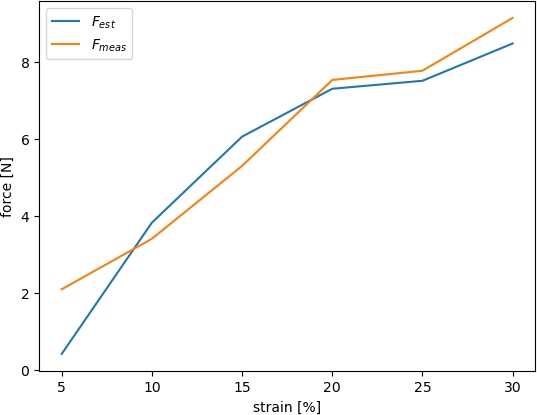
\includegraphics[width=0.7\linewidth]{Figures/CBSR_8p_1_9push_XXstrain_60s_3_force_est_frame31.jpg}
    \caption{Comparing force estimates, $F_{est}$, and actual force measurements, $F_{meas}$, for 5 - 30\% strain centre loading events at $L_0$ for the EIT sensor system for 8 wt\% CBSR}
    \label{fig:stress_est_8p_3}
\end{figure}
% 9wt%
% \begin{figure}[H]
%     \centering
%     \includegraphics[width=8cm]{Figures/CBSR_9p_2_9push_XXstrain_60s_1mA_1_force_est_frame31.jpg}
%     \caption{Force estimations for 5 - 30\% strain centre loading events for the EIT sensor system for CBSR wt 9\% trial 1.}
%     \label{fig:stress_est_9p_1}
% \end{figure}
% \begin{figure}[H]
%     \centering
%     \includegraphics[width=8cm]{Figures/CBSR_9p_2_9push_XXstrain_60s_1mA_2_force_est_frame31.jpg}
%     \caption{Force estimations for 5 - 30\% strain centre loading events for the EIT sensor system for CBSR wt 9\% trial 2.}
%     \label{fig:stress_est_9p_2}
% \end{figure}
\begin{figure}[H]
    \centering
    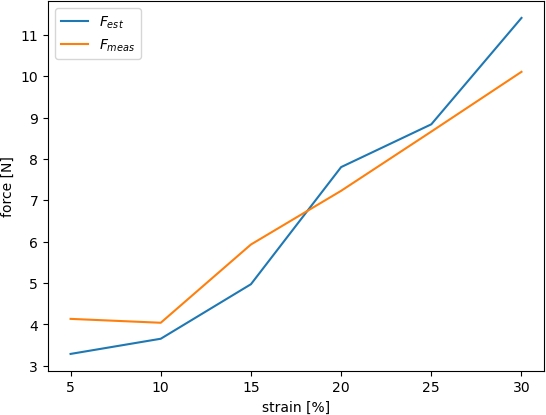
\includegraphics[width=0.7\linewidth]{Figures/CBSR_9p_2_9push_XXstrain_60s_1mA_3_force_est_frame31.jpg}
    \caption{Comparing force estimates, $F_{est}$, and actual force measurements, $F_{meas}$, for 5 - 30\% strain centre loading events at $L_0$ for the EIT sensor system for 9 wt\% CBSR}
    \label{fig:stress_est_9p_3}
\end{figure}
% TODO: Find minimum stress value by determining the stdev for each stress estimate.


\section{Discussion}\label{sec:Discussion}
Potential applications that emulate human-like skin pressure sensing characteristics require a forms of quantification to compare the technology to the specific requirements. This work quantitatively characterises performance metrics to help facilitate that comparison and optimisation process. The sensor developed could be likened to slow acting mechanoreceptors within human skin, such as Meissner's corpuscles and Merkel's discs, which combined can detect static pressure, and high resolution touch. For other EIT-based pressure mapping applications to be realised, the metrics developed in this work are some of the core metrics required to determine which soft sensing domains are suitable and are their limits.

% \subsection{Fabrication}\label{Fabrication3}
% % Fabrication
% The elastic modulus of the 8 wt\% CB was higher than that of the 9 wt\% CB material likely due to a lower degree of curing in the 9 wt\% material. It has been observed in previous literature \citep{Ellingham2021} that larger percentages of CB cause a larger degree of viscoelasticity which is likely due to a lack of cross-linking in the liquid silicone rubber. % TODO?: Cite more sources
% Inhomogeneity was determined when cycling through the inter-electrode resistance of adjacent electrodes, with adjacent inter-electrode resistance varying by up to four times in resistance across all 16 inter-electrode resistance values. This inter-electrode variance in resistance is likely due to inhomogeneity of carbon black particle dispersion. The piezoresistive sensitivity, i.e. the gauge factor, of the sensor CBSR material could be improved by increasing the homogeneity throughout the volume of the sensor material.
% Inhomogeneity gives variable piezoresistivity and viscoelasticity in different regions of the material. 
% Although this inhomogeneity could be determined using absolute EIT reconstruction, it is difficult to determine the ground truth inhomogeneity for the material. -> Could do this by completing a shore hardness test throughout the material and using a bed of nails to determine a resistivity map, then! see if the experiments can be correlated to the shore hardness and resistivity data? Or using TEM or using SAXS to image particle dispersion.

% \subsection{Sensor and Load Applicator Design}\label{Sensor and Load Applicator Design3}
% % Sensor design - shape
% The sensing DUT in this work is configured in a circular shape due to ease of meshing and calculation. This EIT-based sensor could be applied to a range of irregular 2D geometry as shown in several past works \citep{Yoon2017, Zhang2017a}, although this may alter the performance significantly for highly irregular domain geometry.
% % Sensor design - EIT drive
% To test materials with a higher resistivity, a current source with higher driving voltage is required, and thus high voltage multiplexing hardware or high voltage parallel ADC readings. If an increase in EIT data capture frame rate was desired, the use of multiple simultaneous low frequency AC currents could allow for the injection of signals to obtain faster EIT data capture.
% % CFA design
% To obtain a wider variety of compressive touch events types the force applicator head shape could be altered, and a multi-touch force applicator system could be developed such that pressure could be applied to two or more points at the same time with differing periodicity. This data would provide more insight into how well different shapes can be detected.

% \subsection{EIT Solver}\label{EIT Solver3}
% % EIT solver
% A fixed EIT algorithm has been used with fixed parameters in this work. Adaptive optimisation of EIT reconstruction could be completed on a case by case basis further optimising for a range of materials to improve reconstruction time and accuracy. If a real time sensor is required with minimal human perceivable lag, a sample frequency of $\sim$50 Hz is desired similar to that of the consciously perceivable visual frame rate of humans and the upper limit of the frequency response of the rapid acting human mechanoreceptor, the Meissner's corpuscle \citep{Molnar2015}. Currently the device frame rate is limited by the time taken to gather the data for each frame (2.1 s), and more-so by the time taken to complete the EIT image reconstruction of the data (2.5 s). The data measurement time could be improved with sampling hardware. The reconstruction time could be improved with the implementation of EIT algorithm parallelisation and optimisation, and improved computer hardware.

\subsection{Quasi-static Piezoresistivity}\label{Quasi-static Piezoresistivity3}
%  1D stress-strain
%N/A
% 1D quasi-static piezoR
To make a low-frequency response load sensor, a quasi-static piezoresistive linear model was created as shown in Section \ref{sec:1D Material Characterisation2}. However, this model is only valid for sufficiently slow pressure applications or after a sufficiently long time period. This time period is determined by the largest expected steady-state relaxation time for the material, using data gathered in the Temporal Performance Section \ref{sec:Temporal Performance2}.
% 1D transient piezoresistivity 
% N/A

% \subsection{Noise}\label{Noise3}
% % Noise figure
% % The SNR was calculated using the mean vs the stdev for the voltage EIT data and the EIT reconstruction data. Ideally a ground truth model would be used instead of the mean and an offset may be added. But the method used is mathematically legitimate.
% A phenomena called ringing or overshoot has been observed throughout literature \citep{Russo2017, Adler2009} which is the appearance of an artefact around the sensed region blob usually of an opposite sign to the blob. These are generated due to three potential causes. The ringing is generated falsely through the regularisation process. Another reason for the ringing effect seen around the loaded area of the material could be due to the mechanical deformation occurring around the outer edges of the material where the material is in a high shear stress but low compressive stress state. Also the fact that there is a zero crossing shown in Appendix \ref{fig:quasi_r_9p} plot showing that at certain strain the change in conductance goes from negative to positive. Ringing mitigation could be achieved by ignoring any positive changes in resistance and assuming the material is only subject to perpendicular compressive loads and only has a negative change in resistance positively proportional to the compressive stress applied. The pre-processsing in the next section helps minimise these ringing effects, however still could be present and have an effect on the perceived performance metrics. 

\subsection{Pre-processing}\label{Pre-processing3}
% Pre-processing
% The threshold value for the noise threshold mask was often higher than the 25\% threshold mask. Hence, often the 25\% mask would not look dissimilar after the 25\% was applied in noisy data. This behaviour was invariably present in strains $\leq$10\% in 9 wt\% CBSR samples, exhibiting the lower limits of this sensing domain.  
The two steps of a noise threshold mask and a percentage threshold mask successfully filtered noise and EIT reconstruction related noise artefacts. The favoured percentage threshold mask chosen for further metrics testing was 85\% as this gave the lowest average $E_{CoM}$ and $S\!D$ values from the across all strains applied across all nine loading points.

In the experiments often a blob detection from a previous load will be present in a subsequent load, as expected due to the resistive relaxation. Feature detection could be added in future to ensure that only transients similar to those seen in the initial formation of a blob would signify that the blob is to be analysed. Concurrently, each blob could be tracked individually to determine whether it is a noise artefact or an actual sensed region depending on it's behaviour. 
% TODO: Actually ensure the temporal results use threshold % mask.


\subsection{Performance Metrics}\label{Performance Metrics3}
% TODO: Resolution and limitations of the sensor space, time, force.
% Why the performance metrics are good!! :
% TODO: A bit tired now. Check in the morning >>>
To develop sensing domains for future applications, the sensing domains may need take into account certain prior information about the limits of the system.

For example, human hands and feet have some of the highest density of mechanoreceptors in the body. Lower density regions of mechanoreceptors in humans include the back and chest \citep{Kamkim2008}. Higher spatial resolution is require for emulating the pressure mapping of a human hands and feet, compared to the human back and chest. However, the pressure sensing range required by the human hands may be lower than that required by the human feet.

Using this prior information, we can validate the appropriate sensing domain characteristics that give a suitable performance for each different application.
% <<< TODO: A bit tired now. Check in the morning

Depending on the application of the sensor the importance of each temporal, spatial, and force sensing performance metrics could all vary.
% <<< TODO: A bit tired now. Check in the morning

\subsubsection{Spatial Performance}\label{Spaital Performance3}
% Averaging a range of load points in a material with a degree of inhomogeneity meant that a large variance was observed in the spatial metric data across all loads. This variance can be seen in the spatial performance metrics given in \ref{tab:spatial_metrics_stats_8p} and \ref{tab:spatial_metrics_stats_9p}. These results were calculated from all nine different load points across three trials at each load point. 

All spatial performance metrics, $E_{CoM}$, $A_{OL}$, and $S\!D$ are key indicators of whether a loading event has been localised correctly.


% Spatial performance
    % CoM
% Offsets in the $E_{CoM}$ values in certain areas were observed consistently in the same direction over a range of strain values, an artefact generated by a combination of the EIT algorithm and DUT inhomogeneity. Future development could include a vectorised $E_{CoM}$ so sensed regions could be compensated for in different areas of the material. 

    % A_OL
The $A_{OL}$ gives a value out of 100 for a certain detected blob. This value is penalised for false positive and true negative elements that overlap (or not) with the force applicator area.

It is important to note, when a force is applied in an small area of a domain, however a blob has been detected over the majority area of the domain, a $A_{OL}$ value of $\leq$ 50\% will be given although the blob detection could be completely false. Although the detected blob and force applicator are 100\% overlapping the amount of false positive (i.e. blob elements not overlapping with force applicator area) could cover the rest of the DUT, potentially giving a value nearer to 50\% than 0\%. From this it must be recognised that this metric does not represent a linear relationship between $A_{OL}$ and the quality of the reconstruction. So the scale of the $A_{OL}$ value to quality relationship was determined empirically as:
\vspace{-0.4cm}
\begin{center}
    \item 0 $\leq$ $A_{OL}$ $\leq$ 50\% = Likely Poor
    \item 50 $\leq$ $A_{OL}$ $\leq$ 70\% = OK
    \item 70 $\leq$ $A_{OL}$ $\leq$ 100\% = Good
\end{center}

    % SD
The $S\!D$ is the mean square error between the force applicator perimeter and sensed region perimeter taken radially from the force applicator centroid, so will likely be lower with a low $E_{CoM}$ and a higher $A_{OL}$. The closer the $S\!D$ value is to zero the more accurately the shape of the load area applied has been sensed. The $S\!D$ metric is also affected significantly by the quantisation error depending on the mesh coarseness.

Comparing the different percentage threshold masks for the experiment shown in Figure \ref{fig:recon_perform_8p}, it was determined that each percentage mask of 50\%, 75\%, and 85\% gave showed the spatial performance for the $E_{CoM}$, $S\!D$, and $A_{OL}$. However, the standard deviation of these values is comparable to the mean itself therefore looking at the mean performance metric value in each location was shown in Table \ref{tab:spatial_metrics_stats_8p_strain20_loads}. The lowest $E_{CoM}$ was found to be 0.67 $\pm$ 0.41 mm, at $L_2$. The highest $A_{OL}$ value was found to be 87.93 $\pm$ 2.68\%. The lowest $S\!D$ value was found to be 0.12 $\pm$ 0.01 mm$^2$ at $L_1$.

The CBSR 8 wt\% samples gave superior performance metric results than the 9 wt\% samples due to the residual transient effects of previous load events as exemplified in Figure \ref{fig:recon_perform_9p}. This will be mitigated in future by using a blob separation algorithm whereby each sensed-region/blob is given a weighting based on its appearance time, size, decay characteristic, and performance metric values.

The spatial performance metrics are useful for quantifying future testing with irregular load application area shapes and multiple loading events in future testing to validate a variety of irregular and multi-load test cases. Performance metric inconsistencies in the different load locations show that the electromechanical characteristics of the material is varies throughout the material. These metrics would all contribute toward a calibration step to compensate for material inhomogeneity, allowing for a range of materials to be used for the sensing domain.

% could debate that the MSE metric is the best, but this statement breaks for an irregular load applicator head shape.
% TODO: What do the plots mean: e.g. 1) if the CoM error is near or larger than the smallest load applicator spacing then the blob hasn't been detected! or effects for multiple blobs have incurred. 2) if the A_OL is greater than 70% then a it's likely that the blob has been detected as a true positive. If between 50 - 70% there could be a large region of false positive. 3) The SD metric is better the closer it is to zero, however only works well when the force applicator area is a circle and CoM error and A_OL are 'good enough'. 
% TODO: Talk about limitations of the spatial performance metrics - A_OL vs SD for thresh mask = 25% vs 85%.

\subsubsection{Temporal Performance}\label{sec:Temporal Performance3}
% Temporal Performance
Many applications require a minimum frequency response hence a temporal study was completed to characterise the transient effects limiting the speed of the sensor. The study focused on the settling time of transient piezoresistive events in the material for varying strain step inputs. With known PNEC material settling times, a filter could be applied to the output of this sensor to get an estimate of the load applied to the material. 

To aid future inverse modelling and use of PNECs as pressure sensor it is important to understand each transient states of a load, including the loading phase, steady state, or unloading phase. It was found that on average that unloading events had a higher settling time than loading transients for both CBSR 8 and 9 wt\% composites across all strains tested from 5 to 30\%. No clear correlation was found between the settling time of the transient strain events and the strain percentage applied to the material. Mean settling times ranging 29 - 36 s and 29 - 41 s have been observed for the CBSR 8 and 9 wt\% composites respectively. 

% Future work that will increase the reliability of the 2D sensor's temporal results include improvements of EIT image sample rate, the EIT algorithm, and improved post-processing algorithms. To gain more insight into transient characterisation a higher frame for EIT would be beneficial, however for the PNEC material used in this paper the resolution was sufficient for the transient phenomena observed. The EIT algorithm may be acting as a low-pass filter which may be enlarging the settling time relative to the 1D data. 

A different sensing region material could provide a higher frequency response, such as a carbon nanotube silicone composite which has shown a lower settling time in previous works \citep{Zhao2013,Vidhate2010}. Due to the viscoelasticity and elastic rebound in the material the resistance relaxation from previous load applications was often be present in subsequent load events, altering the observed resistance relaxation response. Future algorithms developed would aim to eliminate these previous residual relaxations. 

Often soft materials are inherently viscoelastic like much soft tissue within the human body \citep{Landry2021}, so if soft sensor domains are required with a high frequency response this viscoelasticity will need to be compensated for using this work's performance metrics as a foundation.  

It is important to note that if the homogeneity in the material is highly irregular, regions of the material will have different degrees of piezoresistivity the frequency response of the material is likely to vary considerably. Further research is required into how the different CB wt \% values and their dispersion affect the temporal response of the material.

% TODO: HYPOTHESIS TO PROVE: the relaxation events seen in the 2D EIT reconstructions are correlated to the 1D relaxations events fitted. 
% TODO: Answer - Are the relaxation time constants similar for differences in wt% and strain?
% TODO: Use a different type of material that displays a much smaller degree of the time-dependent transient behaviour

\subsubsection{Localised Force Sensing Performance}\label{sec:Localised Force Sensing Performance3}
The sensor platform gave stress estimates that correlated well with the real stress applied to the material, as seen in Figures \ref{fig:stress_est_8p_3} and \ref{fig:stress_est_9p_3}. These stress estimates were gathered from the steady-state data gathered from the EIT measurements at approximately 1.5x the settling times found in Section \ref{sec:Temporal Performance2} using the algorithm given in Section \ref{sec:Localised Force Sensing Performance2} to ensure the data was at steady state.

Stress relaxation of the composite CBSR material as a whole gives a good indication of macro-mechanical behaviour of the CBSR. It was postulated that the resistance relaxation gives an enhanced insight into the micro(and nano)-structural behaviour of the CBSR composite, because of the different observed behaviours of the CBSR stress and resistive relaxation and also how these relate to different CB weight percentages and their dispersion.


\subsection{Real World Applications, Manufacturability, and Scalability}
Using EIT-based pressure mapping on a larger scale is feasibly as shown by the use of ERT in geophysics \citep{Griffiths1993}. However using the PNEC-based methods given in this work on this scale have not yet been trialled, but potential larger-scale applications include adding a pressure mapping layer under a tennis court to map force exerted by athletes onto a court or a method of measuring foot traffic in buildings and urban areas. The use of the performance metrics discussed in this work would be applicable for both scenarios. 

For the tennis court application, the importance of player location and speed may be more important than detecting the footprint shape and exact force applied to the court surface. This means that the $E_{CoM}$ and decay time values would be more heavily weighted than the $S\!D$ and force values, and hence could be tuned for these characteristics. For the urban floor mat application, the importance of footprint shape and force estimation may give useful insight into the physical demographic of people or animals walking across the mat \cite{Yuan2023}. This may mean that the $S\!D$ and force resolution values are more highly weighted in the design and process.

Larger-scale applications of an EIT-based sensor come with challenges such as, scaling the electronics driving the EIT measurement, fabricating such a large homogeneously piezoresistive domain, and ensuring the reliability in a range of outdoor environmental conditions. Conversely, smaller-scale applications are limited by the conductive particle size in the PNEC. A sensing domain thickness sufficiently larger than the average agglomerate size would be required for reliable EIT mapping and force estimates.

Different forms of tribological wear on the device sensing region would alter the piezoresistive characteristic of the device. Encapsulation of the device could be implemented to minimise wear and increase hermeticity.

The most obvious limitation of this sensor is the frequency response of the material as shown in Appendices \ref{fig:strain_ts_8p_1D} - \ref{fig:strain_ts_9p}, which could be algorithmically filtered or inverse-modelled to be corrected. Else, other more responsive, less viscoelastic materials could be used, and/or a capacitive EIT-based pressure mapping device used to improve the frequency response of this device.

Mass production of an EIT-based sensor would use the performance metrics given in this work to calibrate and quality-check the sensing domain and boundary electrode connections. This work also found that using pin boundary electrodes adds to the durability and stability of electrical connection in this device.

% TODO: Next steps:
% TODO: Could observe how time-dependent viscoelastic phenomena arise with increased strain rate.
% TODO: Try different materials to see limits of other materials and link these limits with material applications.
% TODO: To incorporate the dynamic resistive relaxation effects seen in the material several methods could be used: 
    % 1. A capacitive touch channel on the material domain to distinguish the start and end of a touch event. However this limits the material in terms of what it can distinguish 
    % 2. Differentiating the resistance signal and applying,and applying a different inverse model for material relaxation states, i.e. push and hold state or released state. \citep{Lacasse2010}
    % 3. Train a model that takes into account the resistive relaxation effects using an LTSM or RNNs or one similar to Laaraibi et al \citep{...} 
    % 4. Use a better material lol.
% TODO: Minimum stress of material may not actually be the noise floor seen in the reference frame. As this noise floor may be dynamic and display ringing.

% \subsubsection{Environmental Factors}\label{Environmental Factors3}
% % Sensor environment limitations
% The effects of temperature for this sensor has not been tested and could have a dramatic effect \citep{Lundberg1986}. The effects of water absorbance would need to be tested before being applied in an environment with water exposure and high humidity.

\section{Conclusions}\label{sec:Summary and Conclusions}

% TODO: Mention each subsection and its significance.
% TODO: Include key numbers for spatial, temporal and stress resolution (e.g. XX$\pm$XX)
% TODO: What questions have we asked in the introduction and have they been answered?
%   i.e. How does the carbon black percentage affect the 2D transient phenomena. Relaxation time, blob spread, other reconstruction metrics
% TODO: Has a pressure sensor been developed using methods that have not been combined before?
% TODO: Have we observed time series phenomena in 2D that hasn´t been observed before?
% TODO: How can this be applied to different soft PNECs and what are the key differences for each material?
% TODO: Sentence emphasizing novelty of work to date
% Strains smaller than XX\% cannot be sensed in terms of force reliably by the CBSR 9 wt\% material as shown in Figure \ref{fig:quasi_r_9p}.

An EIT-based piezoresistive sensor using a custom made carbon black silicone rubber composite material has been developed for sensing compressive pressure events and applying performance metrics to obtain the validity of the output EIT images. To be able to apply this EIT-based PNEC pressure sensor to a variety of scenarios, replacing human-like touch, performance metrics has been formed to quantify the sensor's suitability for each application. Sensing domains of 8 and 9 wt\% carbon black silicone rubber have been tested using: 6 strain values, 9 load locations, and 3 trials. From this raw data we have calculated data for: spatial resolution, transient settling time, and force sensor resolution. 

It was shown that the CBSR 8 wt\% sample out performed the CBSR 8wt\% sample in terms of spatial and temporal metrics across a range of experiments. The best performance metrics observed in the CBSR 8 wt\% sample for $E_{CoM}$, $A_{OL}$, and $S\!D$, were 0.67 $\pm$ 0.41 mm, 87.93 $\pm$ 2.68\%, and 0.12 $\pm$ 0.01 mm$^2$ respectively for three different load locations. For the sensor domains tested, average settling times of between 19.0 - 44.5 s and 22.5 - 36.0 s were determined for 8 and 9 wt\% CBSR samples. A quasi-static conductance-force model of the material was developed with an accuracy of  $\pm$ 0.78 and  $\pm$ 0.81 N for a range of strains from a centre load test for 8 and 9 wt\% CBSR respectively.

Using these performance metric data in future work a piezoresistively inhomogeneous sensor domain could be, calibrated to homogenise the apparent domain piezoresistivity, compensated for transient phenomena, and sense loads with a known degree of accuracy. All of these factors contribute to optimising the EIT-based 2D pressure mapping sensor for different applications. The next chapter includes the development of a low-cost, small circuit to discretely capture the EIT data to open up a larger range of mobile and wearable applications. The work shows promise for future use of an EIT-based sensor in a variety of applications requiring a soft sensing domain and non-invasive rigid electrodes.

%\afterpage{\blankpage}